\documentclass[a4paper, 13pt]{article}
\usepackage{fullpage}
\usepackage[utf8]{inputenc}
\usepackage[russian]{babel}

\usepackage{fullpage}
\usepackage{blindtext}
\usepackage{scrextend}
\usepackage{enumitem}
\addtokomafont{labelinglabel}{\sffamily}
\usepackage{hyperref}
\usepackage{parskip}
\usepackage{tikz}
\usepackage{amsmath}
\usepackage{amsfonts}
\usepackage{hyperref}
\usepackage{lscape}
\usepackage{subfig}
\usepackage{url}
\usepackage{geometry}
\usepackage{url}
\usepackage[colorinlistoftodos]{todonotes}

\pagestyle{plain}
\graphicspath{{/}}

\newcommand{\labstablefraction}{1/10}
\newcommand{\labstablescore}{\textwidth * \labstablefraction}
\newcommand{\labstabletask}{\textwidth * (1 - \labstablefraction) - \labstablescore - 0.83cm}

% \geometry{left=2cm}
% \geometry{right=1.5cm}
% \geometry{top=1.5cm}
% \geometry{bottom=1.5cm}

\usepackage{minted}
\usepackage{caption}

\newenvironment{code}{\captionsetup{type=listing}}{}
\DeclareCaptionFont{white}{\color{white}}
\DeclareCaptionFormat{listing}{\colorbox{gray}{\parbox{\textwidth}{#1#2#3}}}
\captionsetup[listing]{format=listing,labelfont=white,textfont=white}

\renewcommand{\theFancyVerbLine}{\sffamily \textcolor[rgb]{1.0,1.0,1.0}{\small \oldstylenums{\arabic{FancyVerbLine}}}}
\setminted[csharp]{linenos=true, baselinestretch=0.8}

\begin{document}

\newpage

\tableofcontents
\newpage

\part{Самостоятельная работа} 
\newpage

\section{Введение}

\graphicspath{{parts/guides/1_introduction/images/}}

\subsection{Рекомендуемые к использованию инструменты}

Для освоения курса разработки оконных приложений для настольных систем Windows с помощью технологии WPF рекомендуется использовать IDE (интегрированную среду разработки) \textbf{Visual Studio Community 2017} с установленными расширениями \textbf{JetBrains ReSharper Ultimate} и \textbf{MVVM Light Toolkit}.

\subsection{Обзор технологии WPF}

Технология WPF (Windows Presentation Foundation) является часть экосистемы платформы .NET и представляет собой подсистему для построения графических интерфейсов для настольных систем Windows.

Одной из особенностей является то, что WPF использует расширяемый язык разметки для приложений (XAML), чтобы предоставить декларативную модель для программирования приложений. XAML основан на языке XML. Таким образом возможно создание пользовательского интерфейса, используя декларативное объявление и/или код на языке C\texttt{\#}.
\todo{Подумать над оформлением}


\newpage
\subsection{Создание проекта}
Давайте начнем изучение нашего курса с создания проекта приложения.

\begin{enumerate}
    \item Откройте \textbf{Visual Studio} и выберите \textbf{файл} (\textbf{File}) > \textbf{Создать} (\textbf{New}) > \textbf{Проект} (\textbf{Project}).
    \item В разделе \textbf{установленные} (\textbf{installed}) выберите подраздел \textbf{Visual C\texttt{\#}}
    \item Затем выберите пункт \textbf{Приложение WPF (.NET Framework)} / \textbf{WPF App (.NET Framework)}
    \item В нижней части окна вы можете указать основные параметры Вашего приложения
    \item Укажите \textbf{имя} (\textbf{name}) приложения (Например, \textit{HelloWorldApp}) и \textbf{путь} (\textbf{location}) для его сохранения
    \item \textbf{Имя решения} (\textbf{solution name}) можно оставить таким же как и \textbf{имя} приложения
    \item Рекомендуется выбрать платформу \textbf{.NET Framework 4.7.1}
    \item Отметьте пункт \textbf{Создать каталог для решения} (\textbf{Create directory for solution})
    \item Если вы хотите использовать систему контроля версий \textbf{Git}, то отметьте пункт \textbf{Добавить в систему управления версиями} (\textbf{Create new Git repository})
    \item Нажмите кнопку \textbf{OK}
\end{enumerate}

\begin{figure}[H]
\centering
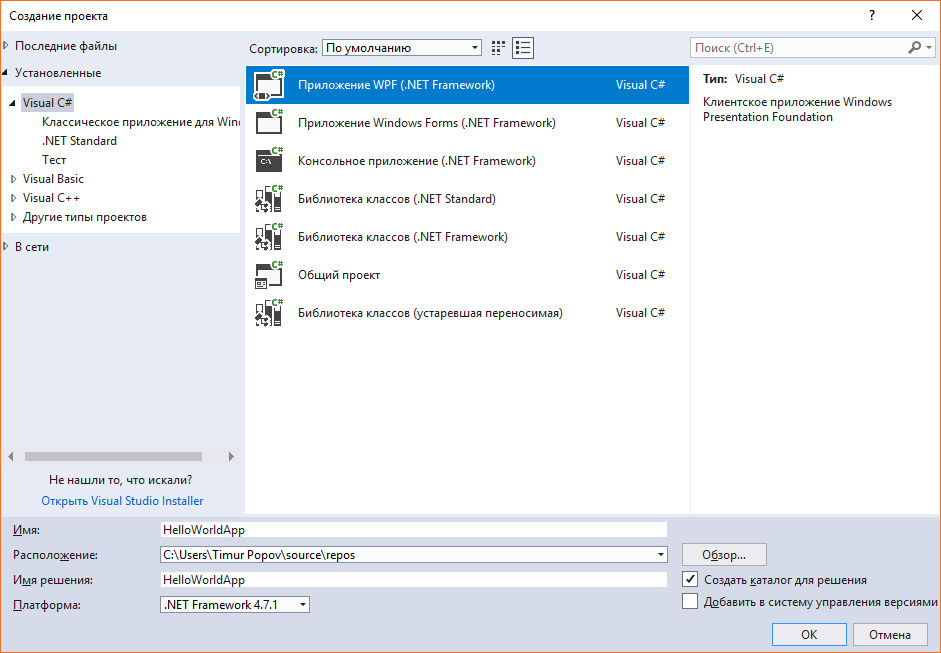
\includegraphics[width=1\textwidth]{introduction_create_project.png}
\end{figure}

\newpage
По умолчанию \textbf{Visual Studio} открывает создает и открывает нам два файла: файл декларативной разметки интерфейса \path{MainWindow.xaml} и файл связанного с разметкой кода \path{MainWindow.xaml.cs}. Файл \path{MainWindow.xaml} имеет два представления: визуальное — в режиме \textbf{WYSIWIG} отображает весь графический интерфейс данного окна приложения, и под ним декларативное объявление интерфейса в \textbf{XAML}. Если мы изменим декларативную разметку, например, определим там кнопку, то эти изменения отображаться в визуальном представлении.

\begin{figure}[H]
\centering
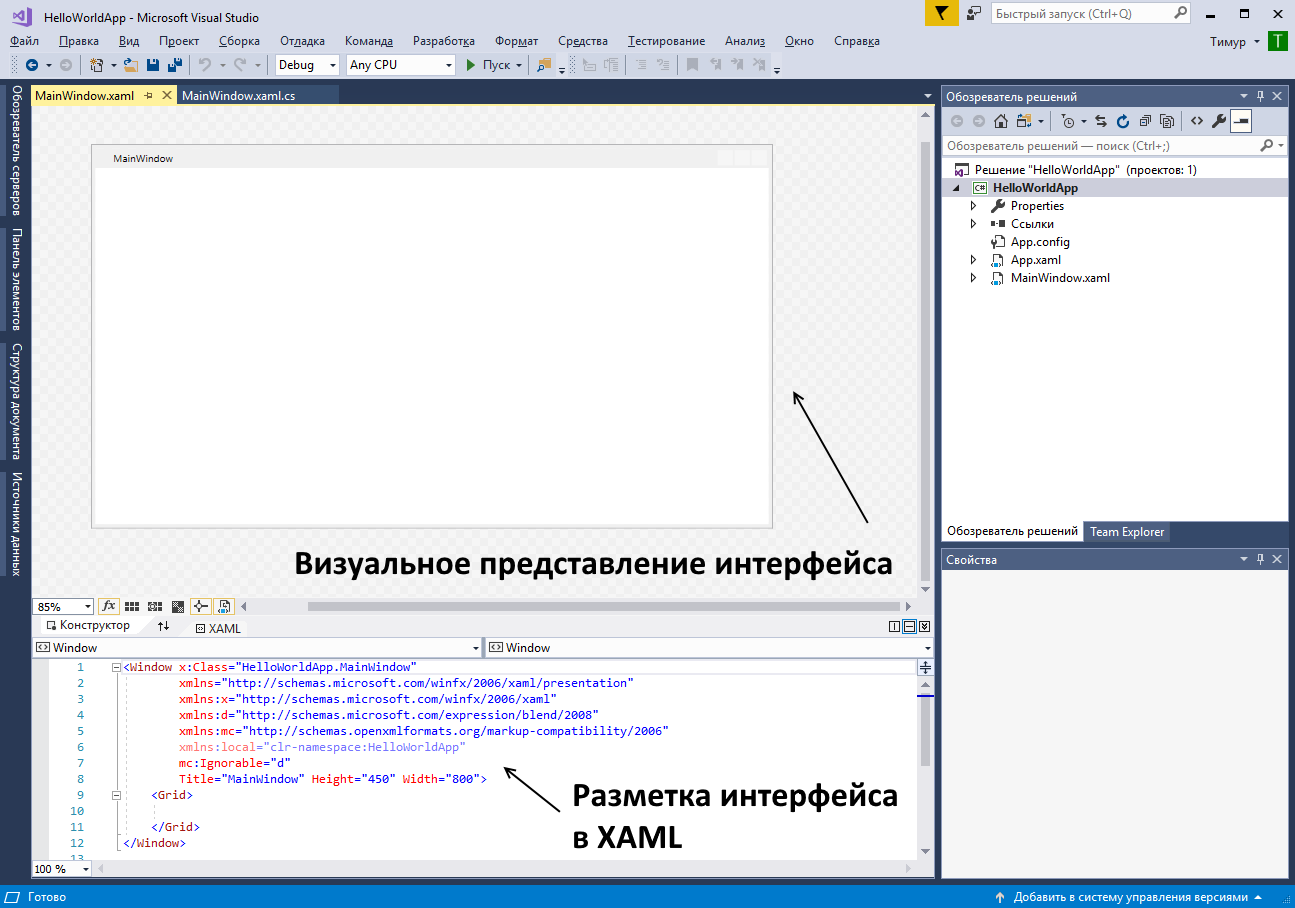
\includegraphics[width=1\textwidth]{introduction_project.png}
\end{figure}

\newpage
\subsection{Знакомство с базовой структурой WPF приложения}

Главным файлом в проекте является \path{App.xaml} и связанный с ним файл кода \path{App.xaml.cs} — это глобальные файлы для всего приложения, определяют его параметры и ресурсы. Так же там указан файл, определяющий главное окно приложения, которое будет открываться при запуске. Это происходит в следующей строке

\begin{minted}{xml}
StartupUri="MainWindow.xaml"
\end{minted}

то есть в данном случае, когда мы запустим приложение, будет создаваться интерфейс из файла \path{MainWindow.xaml}. 

У каждого файла \path{*.xaml} есть парный ему файл \path{*.xaml.cs}, который ещё называется \textbf{Code-Behind}. В нем сокрыта вся внутренняя структура, что позволяет ускорить написание кода и упростить поиск ошибок.

Так же вы обнаружите файл \path{App.confg}, который отвечает за настройку среды CLR и дополнительные параметры Вашего приложения.

\subsection{Основы XAML} \label{XAML_basics}
XAML (eXtensible Application Markup Language) — язык разметки, используемый для инициализации объектов в технологиях на платформе .NET. Применительно к WPF данный язык используется прежде всего для создания пользовательского интерфейса декларативным путем наподобие HTML в веб-программировании. Однако, сводить XAML к одному интерфейсу было бы неверно, и далее на примерах мы это увидим.

XAML — не является обязательной частью приложения, мы можем обходиться без него, создавая все элементы в Code-Behind. Однако использование XAML все-таки несет некоторые преимущества:

\begin{itemize}
\item Возможность отделить графический интерфейс от логики приложения.
\item Компактность, понятность. Код на XAML относительно легко поддерживать.
\end{itemize}

При компиляции приложения в Visual Studio код в XAML-файлах компилируется в бинарное представление, которое называется BAML (Binary Application Markup Language), а затем встраивается в финальную сборку приложения.

При создании нового проекта WPF он уже содержит файлы XAML. Создаваемый по умолчанию в проекте файл \path{MainWindow.xaml} будет иметь следующую разметку:

\begin{minted}{xml}
<Window x:Class="HelloWorldApp.MainWindow"
        xmlns="http://schemas.microsoft.com/winfx/2006/xaml/presentation"
        xmlns:x="http://schemas.microsoft.com/winfx/2006/xaml"
        xmlns:d="http://schemas.microsoft.com/expression/blend/2008"
        xmlns:mc="http://schemas.openxmlformats.org/markup-compatibility/2006"
        xmlns:local="clr-namespace:HelloWorldApp"
        mc:Ignorable="d"
        Title="MainWindow" Height="450" Width="800">
    <Grid></Grid>
</Window>
\end{minted}

Как и в структуре веб-страницы на HTML, здесь есть иерархия элементов. Элементом верхнего уровня является \mintinline{xml}{Window}, который представляет собой окно приложения. При создании других окон в приложении нам придется всегда начинать объявление интерфейса с элемента \mintinline{xml}{Window}.

Элемент \mintinline{xml}{Window} имеет вложенный пустой элемент \mintinline{xml}{Grid}, а также ряд свойств: \mintinline{xml}{Title}, \mintinline{xml}{Width}, \mintinline{xml}{Height}) — заголовок, ширину и высоту окна соответственно.

\subsubsection{Пространства имен XAML}

Чтобы задействовать элементы в XAML, мы подключаем пространства имен. Вторая и третья строчки в коде выше как раз и представляют собой пространства имен, подключаемые в проект по умолчанию. А атрибут \mintinline{xml}{xmlns} представляет специальный атрибут для определения пространства имен в XML.

Так, пространство имен \mintinline{xml}{http://schemas.microsoft.com/winfx/2006/xaml/presentation} содержит описание и определение большинства элементов управления. Так как является пространством имен по умолчанию, то объявляется без всяких префиксов.

\mintinline{xml}{http://schemas.microsoft.com/winfx/2006/xaml} — это пространство имен, которое определяет некоторые свойства XAML, например Name или Key. Используемый префикс \mintinline{xml}{x} в определении \mintinline{xml}{xmlns:x} означает, что те свойства элементов, которые заключены в этом пространстве имен, будут использоваться с префиксом \mintinline{xml}{x}, например \mintinline{xml}{x:Name} или \mintinline{xml}{x:Key}. Это же пространство имен используется уже в первой строчке 

\begin{minted}{xml}
x:Class="XamlApp.MainWindow"
\end{minted}

Здесь создается новый класс \mintinline{csharp}{MainWindow} и соответствующий ему файл кода, куда будет описываться логика для данного окна приложения.

Это два основных пространства имен. Рассмотрим остальные:

\mintinline{xml}{xmlns:d="http://schemas.microsoft.com/expression/blend/2008"} обеспечивает поддержку атрибутов в режиме дизайнера. Это пространство имен преимущественно предназначено для другого инструмента по созданию дизайна на XAML — Microsoft Expression Blend

\mintinline{xml}{xmlns:mc="http://schemas.openxmlformats.org/markup-compatibility/2006"} обеспечивает режим совместимости разметок XAML.

\mintinline{xml}{mc:Ignorable="d"} это выражение позволяет игнорировать парсерам XAML во время выполнения приложения дизайнерские атрибуты из пространства имен с префиксом \mintinline{xml}{d}, то есть из \mintinline{xml}{"http://schemas.microsoft.com/expression/blend/2008"}

\mintinline{xml}{xmlns:local="clr-namespace:HelloWorldApp"} пространство имен текущего проекта. Так как наш проект называется \path{HelloWorldApp}, то простраство имен называется аналогично. Через префикс \mintinline{xml}{local} возмжно получить XAML различные объекты, которые определены в проекте.

Важно понимать, что эти пространства имен не эквивалентны тем пространствам имен, которые подключаются при помощи директивы \mintinline{csharp}{using} в C\texttt{\#}. Так, например,

\mintinline{xml}{"http://schemas.microsoft.com/winfx/2006/xaml/presentation"} 

подключает сразу в проект следующие пространства имен:

\begin{minted}{csharp}
System.Windows
System.Windows.Automation
System.Windows.Controls
System.Windows.Controls.Primitives
System.Windows.Data
System.Windows.Documents
System.Windows.Forms.Integration
System.Windows.Ink
System.Windows.Input
System.Windows.Media
System.Windows.Media.Animation
System.Windows.Media.Effects
System.Windows.Media.Imaging
System.Windows.Media.Media3D
System.Windows.Media.TextFormatting
System.Windows.Navigation
System.Windows.Shapes
System.Windows.Shell
\end{minted}

\subsubsection{Элементы и их атрибуты}
Каждый элемент, как и любой элемент XML, должен иметь открытый и закрытый тег, как в случае с элементом \mintinline{xml}{Window}:

\mintinline{xml}{<Window></Window>}

Либо элемент может иметь сокращенную форму с косой чертой ("слэшем") в конце, наподобие:

\mintinline{xml}{<Window />}

Но в отличие от элементов XML каждый элемент в XAML соответствует определенному классу C\texttt{\#}. Например, элемент \mintinline{xml}{<Button>} соответствует \mintinline{csharp}{System.Windows.Controls.Button}. А свойства этого класса соответствуют атрибутам элемента \mintinline{xml}{<Button>}.

Например, давайте добавим в создаваемую по умолчанию разметку окна (она рассмотрена в \ref{XAML_basics}) менеджер компоновки \mintinline{xml}{StackPanel} (подробнее рассматривается в \ref{panel_definition}), а в него текстовое поле \mintinline{xml}{TextBox} и кнопку \mintinline{xml}{Button}. Для этого мы должны добавить в \mintinline{xml}{Grid} следующее

\begin{minted}{xml}
...
<Grid>
    <StackPanel VerticalAlignment="Center" Margin="50">
        <TextBox x:Name="MagicTextBox" />
        <Button 
            x:Name="MagicButton" 
            Background="Purple" 
            Foreground="White" 
            Content="Click me" 
        />
    </StackPanel>
</Grid>
...
\end{minted}

Элемент \mintinline{xml}{Grid} — это контейнер для других элементов. В нем мы определили контейнер \mintinline{xml}{<StackPanel>}, а уже в нем \mintinline{xml}{<TextBox>} и \mintinline{xml}{<Button>}, текстовое поле и кнопку соответственно.

Определим некоторые свойства для наших элементов. Например, у кнопки здесь определены свойства \mintinline{xml}{x:Name} (имя кнопки), \mintinline{xml}{Background} (фон кнопки), \mintinline{xml}{Foreground} (цвет текста кнопки) и \mintinline{xml}{Content}. Причем, свойство \mintinline{xml}{x:Name} берется в данном случае из пространства имен \mintinline{xml}{"http://schemas.microsoft.com/winfx/2006/xaml"}, которое сопоставляется с префиксом \mintinline{xml}{x}. 
А остальные свойства не используют префиксы, поэтому берутся из основного пространства имен \mintinline{xml}{"http://schemas.microsoft.com/winfx/2006/xaml/presentation"}.

Давайте попробуем добавить в наше приложение немного интерактивности. Для этого кликните 2 раза по кнопке в визуальном конструкторе, после чего откроется файл \path{MainWindow.xaml.cs} и там будет сгененрирован метод \mintinline{csharp}{MagicButton_Click(object, RoutedEventArgs)}.

Добавим в него следующий код, который при нажатии на кнопку будет показывать окно \mintinline{csharp}{MessageBox} с содержимым текстового поля \mintinline{csharp}{TextEdit}.

\begin{minted}{csharp}
private void MagicButton_Click(object sender, RoutedEventArgs e)
{
    MessageBox.Show("Skidaddle skidoodle " + MagicTextBox.Text, "Some magic title");
}
\end{minted}


Скомпилируем и запустим проект (сочетание клавиш Ctrl-F5).


\newpage
\subsection{Функциональная классификация элементов управления WPF}

Ниже перечислены встроенные элементы управления WPF:

\begin{description}[style=nextline]
    \item [Кнопки] \mintinline{xml}{Button} и \mintinline{xml}{RepeatButton}
    \item [Вывод данных] \mintinline{xml}{DataGrid}, \mintinline{xml}{ListView} и \mintinline{xml}{TreeView}
    \item [Вывод и выбор дат] \mintinline{xml}{Calendar} и \mintinline{xml}{DatePicker}
    \item [Диалоговые окна] \mintinline{xml}{OpenFileDialog}, \mintinline{xml}{PrintDialog} и \mintinline{xml}{SaveFileDialog}
    \item [Рукописный ввод] \mintinline{xml}{InkCanvas} и \mintinline{xml}{InkPresenter}
    \item [Документы] \mintinline{xml}{DocumentViewer}, \mintinline{xml}{FlowDocumentPageViewer},     \mintinline{xml}{FlowDocumentReader}, \mintinline{xml}{FlowDocumentScrollViewer} и StickyNoteControl
    \item [Ввод] \mintinline{xml}{TextBox}, \mintinline{xml}{RichTextBox} и \mintinline{xml}{PasswordBox}
    \item [Макет] \mintinline{xml}{Border}, \mintinline{xml}{BulletDecorator}, \mintinline{xml}{Canvas}, \mintinline{xml}{DockPanel}, \mintinline{xml}{Expander}, \mintinline{xml}{Grid}, \mintinline{xml}{GridView}, \mintinline{xml}{GridSplitter}, \mintinline{xml}{GroupBox}, \mintinline{xml}{Panel}, \mintinline{xml}{ResizeGrip}, \mintinline{xml}{Separator}, \mintinline{xml}{ScrollBar}, \mintinline{xml}{ScrollViewer}, \mintinline{xml}{StackPanel}, \mintinline{xml}{Thumb}, \mintinline{xml}{Viewbox}, \mintinline{xml}{VirtualizingStackPanel}, \mintinline{xml}{Window} и \mintinline{xml}{WrapPanel}
    \item [Мультимедиа] \mintinline{xml}{Image}, \mintinline{xml}{MediaElement} и \mintinline{xml}{SoundPlayerAction}
    \item [Меню] \mintinline{xml}{ContextMenu}, \mintinline{xml}{Menu} и \mintinline{xml}{ToolBar}
    \item [Навигация] \mintinline{xml}{Frame}, \mintinline{xml}{Hyperlink}, \mintinline{xml}{Page}, \mintinline{xml}{NavigationWindow} и \mintinline{xml}{TabControl}
    \item [Выбор] \mintinline{xml}{CheckBox}, \mintinline{xml}{ComboBox}, \mintinline{xml}{ListBox}, \mintinline{xml}{RadioButton} и \mintinline{xml}{Slider}
    \item [Информирование пользователя] \mintinline{xml}{AccessText}, \mintinline{xml}{Label}, \mintinline{xml}{Popup}, \mintinline{xml}{ProgressBar}, \mintinline{xml}{StatusBar}, \mintinline{xml}{TextBlock} и \mintinline{xml}{ToolTip}
\end{description}
\section{Контейнеры компоновки}

\graphicspath{{parts/guides/2_managers/images/}}

\subsection{Общая информация о компоновке} \title{panel_definition}

Компоновка (layout) представляет собой процесс размещения элементов внутри контейнера. С помощью неё в WPF осуществляется процесс позиционирования элементов для реализация адаптивной верстки — подход в верстке, при котором элементы приспосабливаются к изменениям размеров контейнера, на котором они расположены.

В WPF компоновка осуществляется при помощи специальных контейнеров

\mintinline{xml}{Grid}, \mintinline{xml}{UniformGrid}, \mintinline{xml}{StackPanel}, \mintinline{xml}{WrapPanel}, \mintinline{xml}{DockPanel} и \mintinline{xml}{Canvas}.

Различные контейнеры могут содержать внутри себя другие контейнеры. Кроме данных контейнеров существует еще ряд элементов, такие как \mintinline{xml}{TabPanel}, которые могут включать другие элементы и даже контейнеры компоновки, однако на саму компоновку не столь влияют в отличие от перечисленных выше.

Каждый из контейнеров наследуется от абстрактного класса \mintinline{csharp}{Panel}, который в свою очередь наследуется от класса \mintinline{csharp}{FrameworkElement}.

При компоновке элементов нежелательно вручную указывать их точные размеры и расположение элементов, так как определение этих параметров задача контейнера.

Процесс компоновки проходит два этапа: измерение (measure) и расстановка (arrange). На этапе измерения контейнер производит измерение предпочтительного для дочерних элементов места. Однако не всегда имеется достаточно места, чтобы расставить все элементы по их предпочтительным размерам, поэтому их размеры приходится усекать. Затем происходит этап непосредственной расстановки дочерних элементов внутри контейнера.

\subsection{\mintinline{xml}{Grid}} \label{Grid_defenition}

\mintinline{xml}{Grid} - контейнер, определяющий адаптивную сетку, которая состоит из строк, определяемых через \mintinline{xml}{RowDefinitions}, и столбцов, определяемых через \mintinline{xml}{ColumnDefinitions}. Пример использование такого контейнера

\begin{minted}{xml}
<Grid>
    <Grid.RowDefinitions>
        <RowDefinition />
        <RowDefinition />
        <RowDefinition />
    </Grid.RowDefinitions>
    <Grid.ColumnDefinitions>
        <ColumnDefinition />
        <ColumnDefinition />
        <ColumnDefinition />
    </Grid.ColumnDefinitions>
    
    <!-- Тут может находиться какой-то код -->
</Grid>
\end{minted}

В данном случае у нас определено 3 строки и 3 столбца.

Чтобы задать позицию элемента управления с привязкой к определенной ячейке \mintinline{xml}{Grid}, в разметке элемента нужно прописать значения свойств \mintinline{xml}{Grid.Column} и \mintinline{xml}{Grid.Row}, тем самым указывая, в каком столбце и строке будет находиться элемент. Кроме того, если мы хотим растянуть элемент управления на несколько строк или столбцов, то можно указать свойства \mintinline{xml}{Grid.ColumnSpan} и \mintinline{xml}{Grid.RowSpan}, как в следующем примере:

\begin{minted}{xml}
<Grid ShowGridLines="True">
    <Grid.RowDefinitions>
        <RowDefinition></RowDefinition>
        <RowDefinition></RowDefinition>
        <RowDefinition></RowDefinition>
    </Grid.RowDefinitions>
    <Grid.ColumnDefinitions>
        <ColumnDefinition></ColumnDefinition>
        <ColumnDefinition></ColumnDefinition>
        <ColumnDefinition></ColumnDefinition>
    </Grid.ColumnDefinitions>
    <TextBlock Grid.Column="0" Grid.Row="0" Text="Столбец 0 Строка 0" />
    <TextBlock Grid.Column="0" Grid.Row="1" Grid.ColumnSpan="3" 
        Text="Объединение трех столбцов, строка 1" 
        VerticalAlignment="Center" 
        HorizontalAlignment="Center" 
        FontSize="40" 
    />
    <TextBlock Grid.Column="2" Grid.Row="2" Text="Строка 2 Столбец 2" />
</Grid>
\end{minted}

В результате получим:

\begin{figure}[H]
\centering
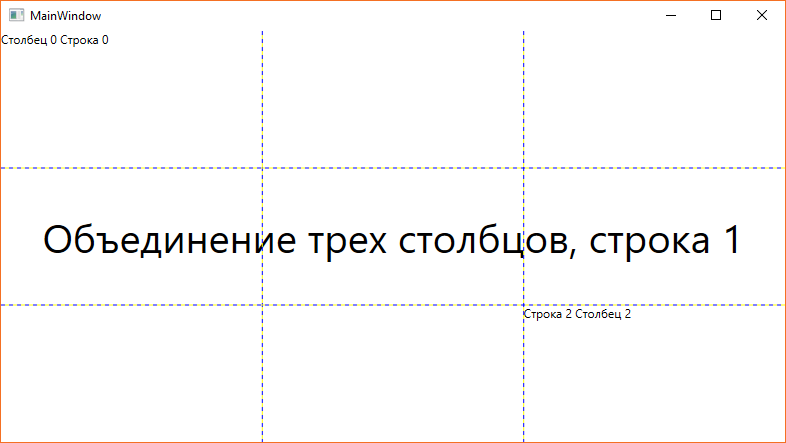
\includegraphics[width=1\textwidth]{manager_grid.png}
\end{figure}


Свойство \mintinline{xml}{ShowGridLines="True"} у элемента \mintinline{xml}{Grid} задает видимость сетки.

При определении строк и столбцов можно указать их размеры. Делается это тремя способами

\begin{description}[style=nextline]
\item [Автоматические размеры] Здесь столбец или строка занимает столько места, сколько им нужно

\begin{minted}{xml}
<ColumnDefinition Width="Auto" />
<RowDefinition Height="Auto" />
\end{minted}

\item [Абсолютные размеры] В данном случае высота и ширина указываются в единицах, независимых от устройства:

\begin{minted}{xml}
<ColumnDefinition Width="150" />
<RowDefinition Height="150" />
\end{minted}

Также абсолютные размеры можно задать в пикселях (\mintinline{xml}{px}), дюймах (\mintinline{xml}{in}), сантиметрах (\mintinline{xml}{cm}) или точках (\mintinline{xml}{pt}):

\begin{minted}{xml}
<ColumnDefinition Width="1 in" />
<RowDefinition Height="10 px" />
\end{minted}

\item [Пропорциональные размеры] Например, ниже задаются два столбца, второй из которых имеет ширину в четверть от ширины первого:

\begin{minted}{xml}
<ColumnDefinition Width="*" />
<ColumnDefinition Width="0.25*" />
\end{minted}

\end{description}


Если строка или столбец имеет высоту, равную \mintinline{xml}{*}, то данная строка или столбец будет занимать все оставшееся место. Если есть несколько сток или столбцов, высота которых равна \mintinline{xml}{*}, то все доступное место делится поровну между всеми такими сроками и столбцами. Также возможно использование коэффициентов (например \mintinline{xml}{0.25*}). При этом все коэффициенты складываются (\mintinline{xml}{коэффициент * аналогичен 1*}) и затем все пространство делится на сумму коэффициентов.

Например, если 3 столбца:

\begin{minted}{xml}
<ColumnDefinition Width="*" />
<ColumnDefinition Width="0.5*" />
<ColumnDefinition Width="1.5*" />
\end{minted}


В этом случае сумма коэффициентов равна \mintinline{csharp}{1* + 0.5* + 1.5* = 3*}. Если сетка имеет ширину 300 единиц, то коэффициент \mintinline{xml}{1*} будет соответствовать пространству \mintinline{csharp}{300 / 3 = 100} единиц. Поэтому первый столбец будет иметь ширину в \mintinline{csharp}{100} единиц, второй \mintinline{csharp}{100 * 0.5 = 50} единиц, а третий \mintinline{csharp}{100 * 1.5 = 150} единиц.

Можно комбинировать все типы размеров. В этом случае от ширины/высоты сетки отнимается ширина/высота столбцов/строк с абсолютными или автоматическими размерами, и затем оставшееся место распределяется между столбцами/строками с пропорциональными размерами.

\subsection{\mintinline{xml}{UniformGrid}}

Аналогичен контейнеру \mintinline{xml}{Grid} контейнер \mintinline{xml}{UniformGrid}, только в этом случае все столбцы и строки одинакового размера и используется упрощенный синтаксис для их определения

\begin{minted}{xml}
<UniformGrid Rows="2" Columns="2">
    <Button Content="Left Top" />
    <Button Content="Right Top" />
    <Button Content="Left Bottom" />
    <Button Content="Right Bottom" />
</UniformGrid>
\end{minted}

\subsection{\mintinline{xml}{StackPanel}}

Это более простой элемент компоновки. Он располагает все элементы в ряд либо по горизонтали, либо по вертикали в зависимости от ориентации.

В данном случае для свойства \mintinline{xml}{Orientation} по умолчанию используется значение \mintinline{xml}{Vertical}, то есть \mintinline{xml}{StackPanel} создает вертикальный ряд, в который помещает все вложенные элементы сверху вниз. Мы также можем задать горизонтальный стек. Для этого нам надо указать свойство \mintinline{xml}{Orientation="Horizontal"}:

\begin{minted}{xml}
<Window x:Class="StackPanelTest.MainWindow"
        xmlns="http://schemas.microsoft.com/winfx/2006/xaml/presentation"
        xmlns:x="http://schemas.microsoft.com/winfx/2006/xaml"
        xmlns:d="http://schemas.microsoft.com/expression/blend/2008"
        xmlns:mc="http://schemas.openxmlformats.org/markup-compatibility/2006"
        xmlns:local="clr-namespace:StackPanelTest"
        mc:Ignorable="d"
        Title="MainWindow" Height="450" Width="800">

    <Grid>
        <Grid.RowDefinitions>
            <RowDefinition Height="Auto" />
            <RowDefinition Height="*" />
        </Grid.RowDefinitions>
        
        <StackPanel Grid.Row="0" Margin="10">
            <Button Background="White" Content="1" />
            <Button Background="Blue" Content="2" />
            <Button Background="Red" Content="3" />
        </StackPanel>

        <StackPanel Grid.Row="1" Margin="10" Orientation="Horizontal">
            <Button Background="White" MinWidth="30" Content="4" />
            <Button Background="Blue" MinWidth="30" Content="5" />
            <Button Background="Red" MinWidth="30" Content="6" />
        </StackPanel>
    </Grid>
</Window>
\end{minted}

\newpage
Результат:

\begin{figure}[H]
\centering
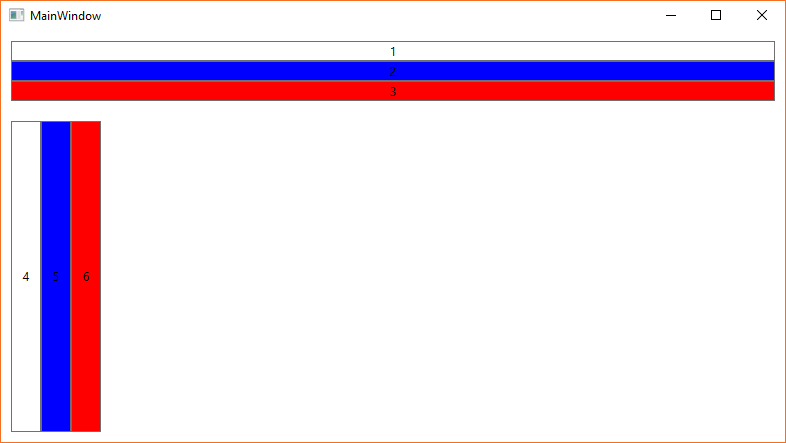
\includegraphics[width=1\textwidth]{manager_stackpanel.png}
\end{figure}

При горизонтальной ориентации все вложенные элементы располагаются слева направо. Если мы хотим, чтобы наполнение стека начиналось справа налево, то нам надо задать свойство \mintinline{xml}{FlowDirection}.

\begin{minted}{xml}
<StackPanel Orientation="Horizontal" FlowDirection="RightToLeft">
\end{minted}

По умолчанию это свойство имеет значение \mintinline{xml}{LeftToRight} — то есть слева направо.

\subsection{\mintinline{xml}{DockPanel}}

Этот контейнер прижимает свое содержимое к определенной стороне внешнего контейнера. Для этого у вложенных элементов надо установить сторону, к которой они будут прижиматься с помощью свойства \mintinline{xml}{DockPanel.Dock}. Например:

В итоге получаем массив кнопок, каждая из которых прижимается к определенной стороне элемента \mintinline{xml}{DockPanel}:

\newpage

\begin{minted}{xml}
<Window x:Class="DockPanelTest.MainWindow"
        xmlns="http://schemas.microsoft.com/winfx/2006/xaml/presentation"
        xmlns:x="http://schemas.microsoft.com/winfx/2006/xaml"
        xmlns:d="http://schemas.microsoft.com/expression/blend/2008"
        xmlns:mc="http://schemas.openxmlformats.org/markup-compatibility/2006"
        xmlns:local="clr-namespace:DockPanelTest"
        mc:Ignorable="d"
        Title="MainWindow" Height="450" Width="800">

    <Grid>
        <DockPanel LastChildFill="True">
            <Button 
                DockPanel.Dock="Top" 
                Background="Orange" 
                Content="Dock Top 1" />
            <Button 
                DockPanel.Dock="Top" 
                Background="Orange" 
                Content="Dock Top 2" />
            <Button 
                DockPanel.Dock="Bottom" 
                Background="IndianRed" 
                Content="Dock Bottom" />
            <Button 
                DockPanel.Dock="Left" 
                Background="Aquamarine" 
                Content="Dock Left 1" />
            <Button 
                DockPanel.Dock="Left" 
                Background="Aquamarine" 
                Content="Dock Left 2" />
            <Button 
                DockPanel.Dock="Right" 
                Background="Azure" 
                Content="Dock Right" />
            <Button 
                Background="DodgerBlue" 
                Content="Dock Center (last)" />
        </DockPanel>
    </Grid>
</Window>
\end{minted}

\newpage
Результат:

\begin{figure}[H]
\centering
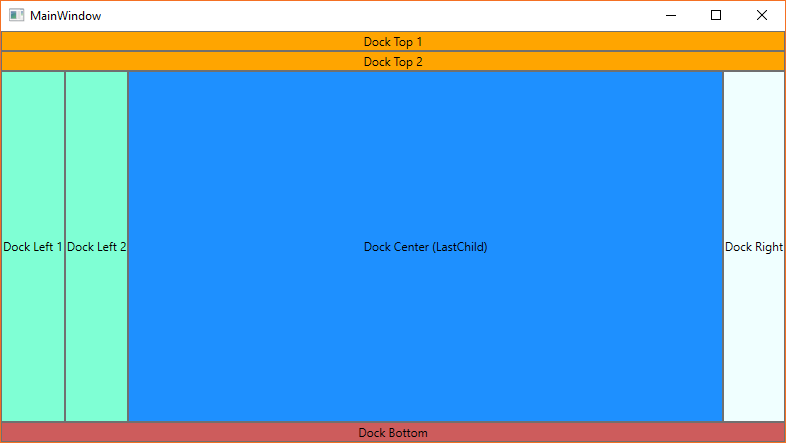
\includegraphics[width=1\textwidth]{manager_dockpanel.png}
\end{figure}


Причем у последней кнопки мы можем не устанавливать свойство \mintinline{xml}{DockPanel.Dock}. Она уже заполняет все оставшееся пространство. Такой эффект получается благодаря установке у \mintinline{xml}{DockPanel} свойства \mintinline{xml}{LastChildFill="True"}, которое означает, что последний элемент заполняет все оставшееся место. Если у этого свойства поменять \mintinline{xml}{True} на \mintinline{xml}{False}, то кнопка прижмется к левой стороне, заполнив только о место, которое ей необходимо.

Контейнер \mintinline{xml}{DockPanel} особенно удобно использовать для создания стандартных интерфейсов, где верхнюю и левую часть могут занимать какие-либо меню, нижнюю — строка состояния, правую — какая-то дополнительная информация, а в центре будет находиться основное содержание.

\subsection{\mintinline{xml}{WrapPanel}}

Эта панель, подобно \mintinline{xml}{StackPanel}, располагает все элементы в одной строке или колонке в зависимости от того, какое значение имеет свойство \mintinline{xml}{Orientation} — \mintinline{xml}{Horizontal} или \mintinline{xml}{Vertical}. Главное отличие от \mintinline{xml}{StackPanel}, если элементы не помещаются в строке или столбце, создаются новые столбец или строка для не поместившихся элементов.

В горизонтальном стеке те элементы, у которых явным образом не установлена высота, будут автоматически принимать высоту самого большого элемента из стека.

В вертикальном стеке элементы, у которых явным образом не указана ширина, автоматически принимают ширину самого широкого элемента.

Мы также можем установить для всех вложенных элементов какую-нибудь определенную ширину (с помощью свойства \mintinline{xml}{ItemWidth}) или высоту (свойство \mintinline{xml}{ItemHeight}).

Расммотрим пример использования \mintinline{xml}{WrapPanel}

\begin{minted}{xml}
<Window x:Class="WrapPanelTest.MainWindow"
        xmlns="http://schemas.microsoft.com/winfx/2006/xaml/presentation"
        xmlns:x="http://schemas.microsoft.com/winfx/2006/xaml"
        xmlns:d="http://schemas.microsoft.com/expression/blend/2008"
        xmlns:mc="http://schemas.openxmlformats.org/markup-compatibility/2006"
        xmlns:local="clr-namespace:WrapPanelTest"
        mc:Ignorable="d"
        Title="MainWindow" Height="450" Width="400">

    <Grid>
        <WrapPanel>
            <Button Background="AliceBlue" Content="1" Width="200" />
            <Button Background="Blue" Content="2" Width="100" />
            <Button Background="Aquamarine" Content="3" Width="100" Height="30" />
            <Button Background="DarkGreen" Content="4" Height="20" />
            <Button Background="LightGreen" Content="5" Width="200" />
            <Button Background="RosyBrown" Content="6" Width="80" />
            <Button Background="GhostWhite" Content="7" />
        </WrapPanel>
    </Grid>
</Window>
\end{minted}

Результат:
\begin{figure}[H]
\centering
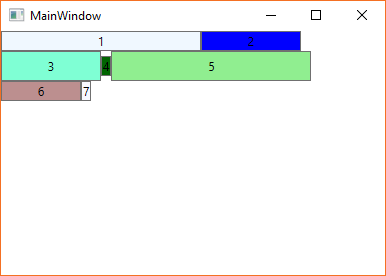
\includegraphics[width=0.5\textwidth]{manager_wrappanel.png}
\end{figure}

\subsection{\mintinline{xml}{Canvas}}

Контейнер \mintinline{xml}{Canvas} является наиболее простым контейнером. Для размещения на нем необходимо указать для элементов точные координаты относительно сторон \mintinline{xml}{Canvas}. Для установки координат элементов используются свойства \mintinline{xml}{Canvas.Left}, \mintinline{xml}{Canvas.Right}, \mintinline{xml}{Canvas.Bottom}, \mintinline{xml}{Canvas.Top}. Например, свойство \mintinline{xml}{Canvas.Left} указывает, на сколько единиц от левой стороны контейнера будет находиться элемент, а свойство \mintinline{xml}{Canvas.Top} сколько единиц ниже верхней границы контейнера находится элемент.

При этом в качестве единиц используются не пиксели, а независимые от устройства единицы, которые помогают эффективно управлять масштабированием элементов. Каждая такая единица равна \mintinline{xml}{1/96} дюйма, и при стандартной установке в \mintinline{xml}{96 dpi} эта независимая от устройства единица будет равна физическому пикселю. В тоже время при работе на других мониторах или при других установленных размеры, установленные в приложении, будут эффективно масштабироваться. Например, при разрешении в \mintinline{xml}{120 dpi} одна условная единица будет равна 1.25 пикселя.

Если элемент не использует свойства \mintinline{xml}{Canvas.Top} и другие, то по умолчанию свойства \mintinline{xml}{Canvas.Left} и \mintinline{xml}{Canvas.Top} будут равны нулю, то есть он будет находиться в верхнем левом углу.

Также надо учитывать, что нельзя одновременно задавать \mintinline{xml}{Canvas.Left} и \mintinline{xml}{Canvas.Right} или \mintinline{xml}{Canvas.Bottom} и \mintinline{xml}{Canvas.Top}. Если подобное произойдет, то последнее заданное свойство не будет учитываться. 

Пример использования:

\begin{minted}{xml}
<Window x:Class="CanvasTest.MainWindow"
        xmlns="http://schemas.microsoft.com/winfx/2006/xaml/presentation"
        xmlns:x="http://schemas.microsoft.com/winfx/2006/xaml"
        xmlns:d="http://schemas.microsoft.com/expression/blend/2008"
        xmlns:mc="http://schemas.openxmlformats.org/markup-compatibility/2006"
        xmlns:local="clr-namespace:CanvasTest"
        mc:Ignorable="d"
        Title="MainWindow" Height="450" Width="600">

    <Grid>
        <Canvas Background="SteelBlue">
            <Rectangle Fill="Orange" 
                Width="150" Height="50" Canvas.Top="20" Canvas.Left="40" />
                
            <Ellipse Fill="Red" 
                Width="150" Height="150" Canvas.Top="60" Canvas.Left="240" />
                
            <Button Content="Button" 
                Width="150" Height="50" Canvas.Bottom="260" Canvas.Right="220" />
        </Canvas>
    </Grid>
</Window>
\end{minted}

\newpage
Результат:
\begin{figure}[H]
\centering
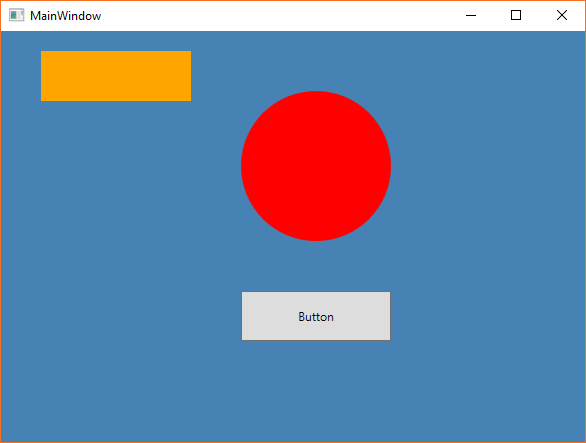
\includegraphics[width=0.8\textwidth]{manager_canvas.png}
\end{figure}
\section{Разработка и оформления элементов управления}
\graphicspath{{parts/guides/3_controls/images/}}

\subsection{Классы \mintinline{csharp}{Brush}, \mintinline{csharp}{Pen}}

\subsubsection{Класс \mintinline{csharp}{Brush}, градиентная заливка}

В примерах ранее были упомянуты такие свойства, как \mintinline{xml}{Background} и \mintinline{xml}{Foreground} и назначение им определенного цвета. Но если посмотреть чуть глубже, то для установки цвета нам нужен объект класса \mintinline{csharp}{System.Media.Brush}. Значение \mintinline{xml}{"Blue"} в данном случае является свойством класса \mintinline{xml}{Brushes}, которое инкапсулирует объект \mintinline{csharp}{SolidColorBrush}. Например, в C\texttt{\#} коде мы можем установить цвет так \mintinline{csharp}{SomeButton.Background = Brushes.Blue}.

Класс \mintinline{csharp}{SolidColorBrush} является кистью или наследником класса \mintinline{csharp}{Brush}, с помощью которого, таким образом, можно устанавливать свойства \mintinline{xml}{Background}, \mintinline{xml}{Foreground} и \mintinline{xml}{BorderBrush}.

WPF поддерживает целый ряд кистей

\begin{description}[style=nextline]
\item [\mintinline{xml}{SolidColorBrush}] Заливает содержимое сплошным цветом.

\begin{minted}{xml}
<Button  Width="160" Height="30" Content="SolidColorBrush">
    <Button.FontSize>18</Button.FontSize>
    <Button.Background>
        <SolidColorBrush Color="Blue" Opacity="0.8" />
    </Button.Background>
    <Button.Foreground>
        <SolidColorBrush Color="White"/>
    </Button.Foreground>
</Button>
\end{minted}

С помощью code-behind кода кисть можно использовать так

\begin{minted}{csharp}
SomeButton.Background = new SolidColorBrush(Colors.Blue);
AnotherOneButton.Background = new SolidColorBrush(Color.FromRgb(207, 255, 255));
\end{minted}

\item [\mintinline{xml}{LinearGradientBrush}] Эта кисть создает плавный переход от одного цвета к другому. Для указания цвета и точек, от которых начинается переход, используется объект GradientStop. Его свойство Color указывает на цвет, а свойство Offset- на точку, с которой начинается переход.

\begin{minted}{xml}
<Button Width="200" Height="50" Content="LinearGradientBrush" >
    <Button.FontSize>18</Button.FontSize>
    <Button.Background>
        <LinearGradientBrush StartPoint="0.5,1" EndPoint="0.5,0">
            <GradientStop Color="White" Offset="0" />
            <GradientStop Color="DarkOrange" Offset="1" />
        </LinearGradientBrush>
    </Button.Background>
    <Button.Foreground>
        <LinearGradientBrush>
            <GradientStop Color="Blue" Offset="1" />
            <GradientStop Color="Green" Offset="0.5" />
            <GradientStop Color="Red" Offset="0" />
        </LinearGradientBrush>
    </Button.Foreground>
</Button>
\end{minted}

С помощью свойств \mintinline{xml}{StartPoint} и \mintinline{xml}{EndPoint} можно определить направление градиента, сделать горизонтальный градиент или градиент под углом.

\item [\mintinline{xml}{RadialGradientBrush}] Эта кисть заполняет элемент радиальным градиентом. Объект \mintinline{xml}{RadialGradientBrush} также имеет коллекцию объектов \mintinline{xml}{GradientStop}, задающих цвет и смещение. Кроме того, он позволяет задавать центр градиента с помощью свойства \mintinline{xml}{GradientOrigin}

\begin{minted}{xml}
<Button Width="200" Height="50" Content="RadialGradientBrush">
    <TextBlock.FontSize>18</TextBlock.FontSize>
    <Button.Background>
        <RadialGradientBrush GradientOrigin="0.4,0.1">
            <GradientStop Color="Black" Offset="1" />
            <GradientStop Color="Blue" Offset="0" />
        </RadialGradientBrush>
    </Button.Background>
    <Button.Foreground>
        <RadialGradientBrush Center="0.4,0.4"  SpreadMethod="Reflect">
            <GradientStop Color="Orange" Offset="1" />
            <GradientStop Color="Red" Offset="0.2" />
        </RadialGradientBrush>
    </Button.Foreground>
</Button>
\end{minted}

Также \mintinline{xml}{RadialGradientBrush} позволяет ограничить область градиента с помощью свойств \mintinline{xml}{RadiusX} и \mintinline{xml}{RadiusY}

\begin{minted}{xml}
<Ellipse Width="60" Height="60"  >
    <Ellipse.Fill>
        <RadialGradientBrush RadiusX="0.6" RadiusY="0.8" GradientOrigin="0.3,0.3">
            <GradientStop Color="Red" Offset="1" />
            <GradientStop Color="White" Offset="0" />
        </RadialGradientBrush>
    </Ellipse.Fill>
</Ellipse>
\end{minted}

\item [\mintinline{xml}{ImageBrush}] Эта кисть использует изображение в качестве фона. Источник устанавливается свойством \mintinline{xml}{ImageSource}. Свойство \mintinline{xml}{Stretch} задает способ заполнения элемента изображением. Если оно равно \mintinline{xml}{Fill} (по умолчанию), то изображение заполняет весь элемент, растягиваясь, если это нужно. Если \mintinline{xml}{Stretch="Uniform"}, то изображение масштабируется пропорционально размеру элемента и по краям могут образоваться пустые места, не заполненные изображением.

\begin{minted}{xml}
<Image Source="image.png" Stretch="Uniform"/>
\end{minted}

Среди прочих свойств \mintinline{xml}{ImageBrush} следует отметить свойство \mintinline{xml}{Viewbox}. Оно применяется для выреза какой-то части изображения. 

\begin{minted}{xml}
<Canvas>
    <Canvas.Background>
        <ImageBrush ImageSource="image.png" Stretch="Uniform"
                    Viewbox="0.5,0.45,0.3,0.2" 
        />
    </Canvas.Background>
</Canvas>
\end{minted}

Его первый параметр служит для установки x-координаты изображения, а второй параметр — y-координаты. Они находятся в пределах от \mintinline{xml}{0} до \mintinline{xml}{1}, и чтобы получить реальные координаты изображения, надо умножить первый параметр на ширину, а второй параметр — на высоту изображения. Третий и четвертый параметр указывают соответственно на ширину и высоту вырезаемого изображения. Так ниже в примере, начальная точка выреза изображения имеет координаты: \mintinline{xml}{0.5 * ширина_изображения}, \mintinline{xml}{0.45 * высота_изображения}. Вырезается 30\% от оставшейся ширины и 20\% от оставшейся длины.

\mintinline{xml}{ImageBrush} также позволяет нам многократно отобразить изображение на элементе и проделывать с ним некоторые преобразования. Для этого класс \mintinline{xml}{ImageBrush} имеет свойство \mintinline{xml}{Viewport}. Оно похоже на \mintinline{xml}{Viewbox}, также задает четыре параметра, только они указывают на координаты прямоугольника \mintinline{xml}{Viewbox} на элементе управления. Первый и второй параметр указывают на начальную координату этого прямоугольника, а третий и четвертый — на конечную точку. Реальные координаты получаются путем умножения параметров на длину и ширину элемента.

Кроме того, свойство \mintinline{xml}{TileMode} позволяет задать режим заполнения элемента изображением. Оно имеет четыре варианта:

\begin{description}[style=nextline]
\item [\mintinline{xml}{Tile}] Изображение многократно повторяется на элементе, пока не заполнит все пространство.
\item [\mintinline{xml}{FlipX}] Изображение повторяется по оси X, и каждый второй столбец является зеркальным отображением предыдущего.
\item [\mintinline{xml}{FlipY}] Изображение повторяется по оси Y, и каждая вторая строка является зеркальным отображением предыдущей.
\item [\mintinline{xml}{FlipXY}] Каждое изображение зеркально отображается как по оси Х, так и по оси Y.
\item [\mintinline{xml}{None}] Создается единичное изображение (по умолчанию)
\end{description}

Пример использования \mintinline{xml}{TileMode}
\begin{minted}{xml}
<Grid.Background>
    <ImageBrush ImageSource="D:\Images\Image.jpg"
                Viewport="0,0,0.25,0.25" TileMode="FlipXY" />
</Grid.Background>
\end{minted}

\item [\mintinline{xml}{DrawingBrush}] С помощью свойства \mintinline{xml}{Drawing} определяет рисунок, включающий: геометрические фигуры, другие элементы и т.д., служащее заполнителем. Он использует те же свойства, что и \mintinline{xml}{ImageBrush}: \mintinline{xml}{Viewport} и \mintinline{xml}{Viewbox}.

\mintinline{xml}{ImageDrawing} — заполнителем кисти является изображение.

\mintinline{xml}{GeometryDrawing} — кисть формируется на основе рисунка, составленного каким-нибудь геометрическим примитивом (прямоугольником, линией, эллипсом)

\mintinline{xml}{VideoDrawing} — кисть формируется на основе видеоресурса.

\mintinline{xml}{GlyphRunDrawing}

При необходимости сочетания нескольких вариантов, используется свойство \mintinline{xml}{DrawingGroup} класса \mintinline{xml}{Drawing}.

\begin{minted}{xml}
<DrawingBrush TileMode="FlipXY" Viewport="0,0,0.25,0.25">
    <DrawingBrush.Drawing>
        <DrawingGroup>
            <GeometryDrawing Brush="Aquamarine">
                <GeometryDrawing.Pen>
                    <Pen Brush="Black" />
                </GeometryDrawing.Pen>
                <GeometryDrawing.Geometry>
                    <EllipseGeometry RadiusX="30" RadiusY="30" 
                                     Center="150,125" />
                </GeometryDrawing.Geometry>
            </GeometryDrawing>
            <GeometryDrawing Brush="Aquamarine">
                <GeometryDrawing.Pen>
                    <Pen Brush="Black" />
                </GeometryDrawing.Pen>
                <GeometryDrawing.Geometry>
                    <LineGeometry EndPoint="150,125" />
                </GeometryDrawing.Geometry>
            </GeometryDrawing>
        </DrawingGroup>
    </DrawingBrush.Drawing>
</DrawingBrush>
\end{minted}

\item [\mintinline{xml}{VisualBrush}] Эта кисть при помощи свойства \mintinline{xml}{Visual} создает привязку к определенному элементу, копируя весь его фон или его часть.

VisualBrush, как и кисти \mintinline{xml}{DrawingBrush} и \mintinline{xml}{ImageBrush}, обладает свойствами \mintinline{xml}{Viewport}, \mintinline{xml}{Viewbox} и \mintinline{xml}{TileMode}, позволяющие проводить все те же преобразования, что были рассмотрены для этих кистей

\begin{minted}{xml}
<Grid Background="Lavender">
    <Button Name="SomeButton" Content="VisualBrush" 
            Background="Black" FontWeight="Black" Foreground="White" 
            HorizontalAlignment="Center" VerticalAlignment="Top"
            Width="100" Height="30"/>
    <TextBlock HorizontalAlignment="Center" VerticalAlignment="Center"
               Width="120" Height="35">
        <TextBlock.Background>
            <VisualBrush Visual="{Binding ElementName=SomeButton}" />
        </TextBlock.Background>
    </TextBlock>
    <TextBlock HorizontalAlignment="Center" VerticalAlignment="Bottom"
               Width="140" Height="50">
        <TextBlock.Background>
            <VisualBrush Visual="{Binding ElementName=SomeButton}" 
                         Viewbox="0.1,0.1,0.3,0.7" />
        </TextBlock.Background>
    </TextBlock>
</Grid>
\end{minted}

\end{description}

Использования различных вариантов кистей:
\begin{figure}[H]
\centering
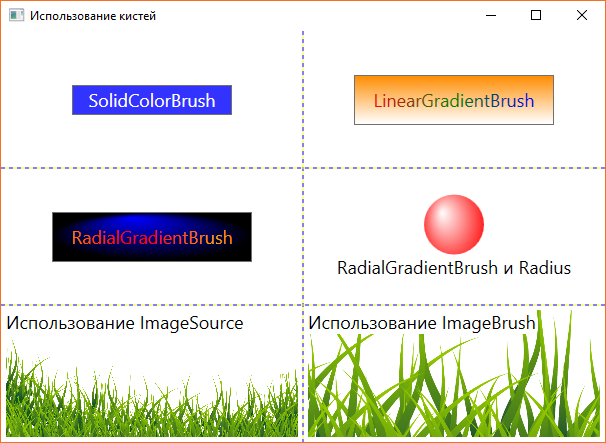
\includegraphics[width=1\textwidth]{brushes.png}
\end{figure}


\newpage
\subsubsection{Класс \mintinline{xml}{Pen}}

В параграфе выше мы так же использовали класс \mintinline{xml}{Pen}. При его использовании мы указывали свойства \mintinline{xml}{Brush} и \mintinline{xml}{Thickness}, что позволяло описывать способ рисования контура фигуры. Но в классе \mintinline{xml}{Pen} определены и другие свойства для более точного управления внешним видом

\begin{description}[style=nextline]

\item [\mintinline{xml}{StartLineCap} и \mintinline{xml}{EndLineCap}] Описывает открытый конец отрезка и может принимать значения, определенные в перечислении \mintinline{xml}{PenLineCap}: \mintinline{xml}{Flat} (плоский, по умолчанию), \mintinline{xml}{Square}, \mintinline{xml}{Round} и \mintinline{xml}{Triangle}. Вид линии в точке соединения двух отрезков управляется свойством \mintinline{xml}{LineJoin}.

\item [\mintinline{xml}{LineJoin}] Описывает способ соединения отрезков в углах ломаной. Может принимать значения из перечисления \mintinline{xml}{PenLineJoin}: \mintinline{xml}{Miter} (по умолчанию), \mintinline{xml}{Round} и \mintinline{xml}{Bevel}. Отдельное свойство \mintinline{xml}{MiterLimit} определяет, насколько выступает уголок соединения типа \mintinline{xml}{Miter}. Если эту длину не ограничить, то для острых углов выступ может оказаться очень большим. По умолчанию принимается значение \mintinline{xml}{10}.

\item [\mintinline{xml}{DashStyle}] Описывает стили линии, рисуемой пером (она необязательно сплошная). Значением этого свойства должен быть объект типа \mintinline{xml}{DashStyle}. Начертание конечных точек штриха можно регулировать свойством \mintinline{xml}{DashCap} класса \mintinline{xml}{Реп}. Оно аналогично свойствам \mintinline{xml}{StartLineCap} и \mintinline{xml}{EndLineCap}, только по умолчанию равно \mintinline{xml}{Square}, а не \mintinline{xml}{Flat}.

\end{description}


Рассмотрим подробнее класс \mintinline{xml}{DashStyle}. В нем имеется свойство \mintinline{xml}{Dashes}. Это простая коллекция \mintinline{xml}{DoubleCollection}, в которой хранится последовательность чисел, представляющих длины штрихов и промежутков между ними. В нечетных элементах находятся длины штрихов (относительно толщины пера), а в четных — длины промежутков. Заданная последовательность повторяется до бесконечности. В классе \mintinline{xml}{DashStyle} имеется также свойство \mintinline{xml}{Offset} типа \mintinline{csharp}{double}, определяющее, где начинает рисоваться последовательность. Странность поведения \mintinline{xml}{DashStyle} заключается в том, что поскольку свойство \mintinline{xml}{DashCap} по умолчанию равно \mintinline{xml}{Square}, то штрих получается длиннее промежутка с точно таким же числовым значением. Более того, для длины штриха вполне можно задать значение \mintinline{xml}{0}, и тогда она окажется равной толщине пера. 

Имеется еще класс \mintinline{xml}{DashStyles}, и в его статическом свойстве \mintinline{xml}{DashStyle} определены некоторые типичные варианты начертания штрихпунктирных линий. Например, можно выбрать вариант \mintinline{xml}{DashDotDot}

\begin{minted}{xml}
<Pen Brush="Black" Thickness="10" DashStyle="{x:Static DashStyles.DashDotDot}" />
\end{minted}

\newpage
\begin{minted}{xml}
<Image>
<Image.Source>
    <DrawingImage>
        <DrawingImage.Drawing>
            <DrawingGroup>
                <!-- Тело -->
                <GeometryDrawing Brush="Orange" Geometry="
                    M 240,250
                    C 200,375 200,250 175,200
                    C 100,400 100,250 100,200
                    C 0,350 0,250 30,130
                    C 75,0 100,0 150,0
                    C 200,0 250,0 250,150 Z"/>
                
                <!-- Глаза -->
                <GeometryDrawing Brush="Black">
                    <GeometryDrawing.Pen>
                        <Pen Brush="White" Thickness="10"/>
                    </GeometryDrawing.Pen>
                    <GeometryDrawing.Geometry>
                        <GeometryGroup>
                            <!-- Левый глаз -->
                            <EllipseGeometry RadiusX="15" RadiusY="15" Center="95,95"/>
                            <!-- Правый глаз -->
                            <EllipseGeometry RadiusX="15" RadiusY="15" Center="170,105"/>
                        </GeometryGroup>
                    </GeometryDrawing.Geometry>
                </GeometryDrawing>
                
                <!-- Рот-->
                <GeometryDrawing>
                    <GeometryDrawing.Pen>
                        <Pen Brush="Black" StartLineCap="Round" EndLineCap="Round" 
                        Thickness="10"/>
                    </GeometryDrawing.Pen>
                    <GeometryDrawing.Geometry>
                        <LineGeometry StartPoint="75,160" EndPoint="175,150"/>
                    </GeometryDrawing.Geometry>
                </GeometryDrawing>
            </DrawingGroup>
        </DrawingImage.Drawing>
    </DrawingImage>
</Image.Source>
</Image>
\end{minted}

\newpage
Полученный результат:
\begin{figure}[H]
\centering

\includegraphics[width=0.75\textwidth]{ghost.png}
\end{figure}

\subsection{Ресурсы}

\subsubsection{Общая концепция}
В .NET Framework встроена общая инфраструктура пакетирования и доступа к ресурсам — частям приложения или компонента, отличным от кода. К ним относятся, например, растровые изображения, шрифты, аудио и видеофайлы и тому подобное. Как и во многих других случаях, WPF не только пользуется базовой системой ресурсов .NET, но и немного расширяет ее. В WPF поддерживается два разных вида ресурсов: бинарные и логические. Мы разберем логические, так как они нам наиболее интересны.

В чем смысл использования ресурсов? Они повышают эффективность: мы можем определить один раз какой-либо ресурс и затем многократно использовать его в различных местах приложения. В связи с этим улучшается поддержка - если возникнет необходимость изменить ресурс, достаточно это сделать в одном месте, и изменения произойдут глобально в приложении.

Логические ресурсы представляют собой произвольные объекты .NET, хранящиеся в свойстве элемента \mintinline{xml}{Resources}. Обычно предполагается, что таким ресурсом смогут сообща пользоваться все потомки данного элемента. Свойство \mintinline{xml}{Resources}  определено в базовых классах \mintinline{xml}{FrameworkElement} и \mintinline{xml}{FrameworkContentElement}, а занчит, оно есть в большинстве классов WPF. В качетсве таких ресурсов часто выступает стили, либо поставщики данных.

Рассмотрим простой пример, показывающий удобство использования логических ресурсов. Предположим нам нужно создать панель с 5 кнопками. Каждая кнопка должна быть желтой, с красной обводкой и белым текстом. Тогда решение без использования ресурсов будет выглядеть так:

\newpage
\begin{minted}{xml}
<Window x:Class="HelloWorldApp.MainWindow"
        xmlns="http://schemas.microsoft.com/winfx/2006/xaml/presentation"
        xmlns:x="http://schemas.microsoft.com/winfx/2006/xaml"
        xmlns:d="http://schemas.microsoft.com/expression/blend/2008"
        xmlns:mc="http://schemas.openxmlformats.org/markup-compatibility/2006"
        xmlns:local="clr-namespace:HelloWorldApp"
        mc:Ignorable="d"
        Title="MainWindow" Height="450" Width="620">

    <Grid>
        <DockPanel Background="SteelBlue">
            <StackPanel 
                DockPanel.Dock="Top" Orientation="Horizontal" 
                HorizontalAlignment="Center" Margin="10" >
                <Button
                    MinWidth="100" Content="Test 1" 
                    BorderBrush="Red" BorderThickness="3"
                    Background="Orange" Foreground="White"
                    FontWeight="Bold" />
                <Button
                    MinWidth="100" Content="Test 2" 
                    BorderBrush="Red" BorderThickness="3"
                    Background="Orange" Foreground="White"
                    FontWeight="Bold" />
                    
                <Button 
                    MinWidth="100" Content="Test 3" 
                    BorderBrush="Red" BorderThickness="3"
                    Background="Orange" Foreground="White" 
                    FontWeight="Bold" />
                    
                <Button 
                    MinWidth="100" Content="Test 4" 
                    BorderBrush="Red" BorderThickness="3"
                    Background="Orange" Foreground="White"
                    FontWeight="Bold" />
                
                <Button 
                    MinWidth="100" Content="Test 5" 
                    BorderBrush="Red" BorderThickness="3"
                    Background="Orange" Foreground="White"
                    FontWeight="Bold" />
            </StackPanel>
            <TextBox/>
        </DockPanel>
    </Grid>
</Window>
\end{minted}

\newpage
Результат:
\begin{figure}[H]
\centering
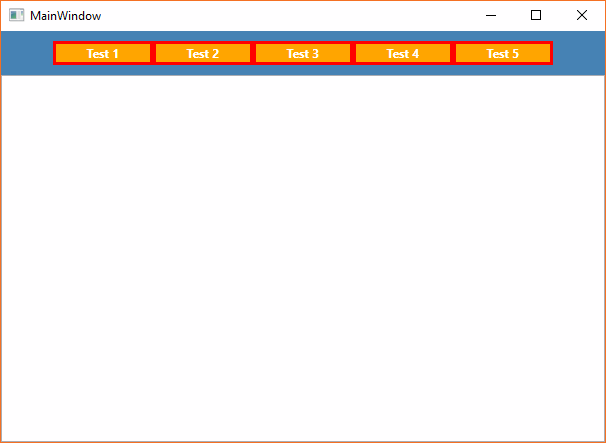
\includegraphics[width=1\textwidth]{resources_without.png}
\end{figure}

Предположим, что нам понадобилось изменить фон у кнопок на желтый, а обводку сделать тонкой красной линией. Здесь на помощь и приходят ресурсы. Обновим пример:

\begin{minted}{xml}
<Window x:Class="HelloWorldApp.MainWindow"
        xmlns="http://schemas.microsoft.com/winfx/2006/xaml/presentation"
        xmlns:x="http://schemas.microsoft.com/winfx/2006/xaml"
        xmlns:d="http://schemas.microsoft.com/expression/blend/2008"
        xmlns:mc="http://schemas.openxmlformats.org/markup-compatibility/2006"
        xmlns:local="clr-namespace:HelloWorldApp"
        xmlns:system="clr-namespace:System;assembly=mscorlib"
        mc:Ignorable="d"
        Title="MainWindow" Height="450" Width="620">

    <Window.Resources>
        <SolidColorBrush x:Key="ButtonBackgroundBrush">Yellow</SolidColorBrush>
        <SolidColorBrush x:Key="ButtonForegroundBrush">Red</SolidColorBrush>
        <SolidColorBrush x:Key="ButtonBorderBrush">Red</SolidColorBrush>
        <Thickness x:Key="ButtonBorderThinkness">1</Thickness>
        <FontWeight x:Key="ButtonFontWeight">Light</FontWeight>
    </Window.Resources>
    
    <Grid>
        <DockPanel Background="SteelBlue">
            <StackPanel 
                DockPanel.Dock="Top" Orientation="Horizontal" 
                HorizontalAlignment="Center" Margin="10" >
                <Button
                    MinWidth="100" Content="Test 1" 
                    BorderBrush="{StaticResource ButtonBorderBrush}"
                    BorderThickness="{StaticResource ButtonBorderThinkness}"
                    Background="{StaticResource ButtonBackgroundBrush}"
                    Foreground="{StaticResource ButtonForegroundBrush}"
                    FontWeight="{StaticResource ButtonFontWeight}" />

                <Button
                    MinWidth="100" Content="Test 2" 
                    BorderBrush="{StaticResource buttonBorderBrush}"
                    BorderThickness="{StaticResource ButtonBorderThinkness}"
                    Background="{StaticResource ButtonBackgroundBrush}"
                    Foreground="{StaticResource ButtonForegroundBrush}"
                    FontWeight="{StaticResource ButtonFontWeight}" />

                <Button
                    MinWidth="100" Content="Test 3" 
                    BorderBrush="{StaticResource buttonBorderBrush}"
                    BorderThickness="{StaticResource ButtonBorderThinkness}"
                    Background="{StaticResource ButtonBackgroundBrush}"
                    Foreground="{StaticResource ButtonForegroundBrush}"
                    FontWeight="{StaticResource ButtonFontWeight}" />

                <Button
                    MinWidth="100" Content="Test 4" 
                    BorderBrush="{StaticResource buttonBorderBrush}"
                    BorderThickness="{StaticResource ButtonBorderThinkness}"
                    Background="{StaticResource ButtonBackgroundBrush}"
                    Foreground="{StaticResource ButtonForegroundBrush}"
                    FontWeight="{StaticResource ButtonFontWeight}" />

                <Button
                    MinWidth="100" Content="Test 5" 
                    BorderBrush="{StaticResource buttonBorderBrush}"
                    BorderThickness="{StaticResource ButtonBorderThinkness}"
                    Background="{StaticResource ButtonBackgroundBrush}"
                    Foreground="{StaticResource ButtonForegroundBrush}"
                    FontWeight="{StaticResource ButtonFontWeight}" />
            </StackPanel>
            <TextBox/>
        </DockPanel>
    </Grid>
</Window>
\end{minted}

Результат:
\begin{figure}[H]
\centering
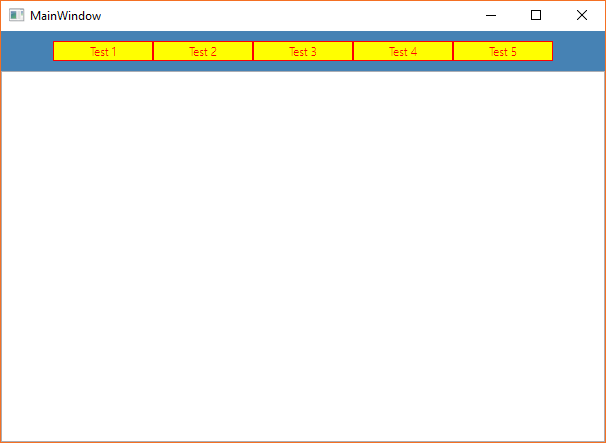
\includegraphics[width=1\textwidth]{resources_step1.png}
\end{figure}

Теперь мы можем отредактировать код только в 1 месте, чтобы изменить все кнопки. Попробуем применить стили, чтобы избавиться от дублирования:

\newpage

\begin{minted}{xml}
<Window x:Class="HelloWorldApp.MainWindow"
        xmlns="http://schemas.microsoft.com/winfx/2006/xaml/presentation"
        xmlns:x="http://schemas.microsoft.com/winfx/2006/xaml"
        xmlns:d="http://schemas.microsoft.com/expression/blend/2008"
        xmlns:mc="http://schemas.openxmlformats.org/markup-compatibility/2006"
        xmlns:local="clr-namespace:HelloWorldApp"
        xmlns:system="clr-namespace:System;assembly=mscorlib"
        mc:Ignorable="d"
        Title="MainWindow" Height="450" Width="620">

    <Window.Resources>
        <SolidColorBrush x:Key="ButtonBackgroundBrush">Yellow</SolidColorBrush>
        <SolidColorBrush x:Key="ButtonForegroundBrush">Red</SolidColorBrush>
        <SolidColorBrush x:Key="ButtonBorderBrush">Red</SolidColorBrush>

        <Thickness x:Key="ButtonBorderThinkness">1</Thickness>
        <FontWeight x:Key="ButtonFontWeight">Light</FontWeight>

        <Style TargetType="{x:Type Button}" x:Key="CustomButton">
            <Setter Property="Background" Value="{StaticResource ButtonBackgroundBrush}"/>
            <Setter Property="Foreground" Value="{StaticResource ButtonForegroundBrush}"/>
            <Setter Property="BorderBrush" Value="{StaticResource ButtonBorderBrush}"/>
            <Setter Property="BorderThickness" Value="{StaticResource ButtonBorderThinkness}"/>
            <Setter Property="FontWeight" Value="{StaticResource ButtonFontWeight}"/>
            <Setter Property="MinWidth" Value="100" />
        </Style>
    </Window.Resources>
    
    <Grid>
        <DockPanel Background="SteelBlue">
            <StackPanel 
                DockPanel.Dock="Top" Orientation="Horizontal" 
                HorizontalAlignment="Center" Margin="10" >
                <Button Style="{StaticResource CustomButton}" Content="Test 1" />
                <Button Style="{StaticResource CustomButton}" Content="Test 2" />
                <Button Style="{StaticResource CustomButton}" Content="Test 3" />
                <Button Style="{StaticResource CustomButton}" Content="Test 4" />
                <Button Style="{StaticResource CustomButton}" Content="Test 5" />
            </StackPanel>
            <TextBox/>
        </DockPanel>
    </Grid>
</Window>
\end{minted}

Результат аналогичен показанному выше, но мы получили решение, которое можно легко переиспользовать. Теперь создать кнопку с аналогичным стилем стало проще.


\subsubsection{Статические и динамические ресурсы}
В примерах выше мы использовали статические ресурсы (\mintinline{xml}{StaticResource}). Рассмотрим, для чего используются динамические ресурсы (\mintinline{xml}{DynamicResource}) и в чем заключаются их отличия. 

Итак, статические ресурсы устанавливается только один раз. А динамические ресурсы могут меняться в течение работы программы. Например, у нас есть ресурс кисти:

\begin{minted}{xml}
<SolidColorBrush Color="LightGray" x:Key="buttonBrush" />
\end{minted}

Для установки ресурса в качестве статического используется выражение \mintinline{xml}{StaticResource}:

\begin{minted}{xml}	
<Button 
    MaxWidth="80" MaxHeight="40" 
    Content="OK" Background="{StaticResource buttonBrush}" />
\end{minted}

Для установки ресурса как динамического применяется выражение \mintinline{xml}{DynamicResource}:

\begin{minted}{xml}
<Button 
    MaxWidth="80" MaxHeight="40" 
    Content="OK" Background="{DynamicResource buttonBrush}" />
\end{minted}

Причем один и тот же ресурс может быть и статическим и динамическим. Чтобы посмотреть различие между ними, добавим к кнопке обработчик нажатия:

\begin{minted}{xml}
<Button x:Name="button1" MaxWidth="80" MaxHeight="40" Content="OK"
        Background="{DynamicResource buttonBrush}"  Click="Button_Click" />
\end{minted}
        
А в файле кода определим в этом обработчике изменение ресурса:

\begin{minted}{csharp}
private void Button_Click(object sender, RoutedEventArgs e)
{
    this.Resources["buttonBrush"] = new SolidColorBrush(Colors.LimeGreen);
}
\end{minted}

И если после запуска мы нажмем на кнопку, то ресурс изменит свой цвет, что приведет к изменению цвета кнопки. Если бы ресурс был бы определен как статический, то изменение цвета кисти никак бы не повлияло на цвет фона кнопки.

В то же время надо отметить, что мы все равно может изменить статический ресурс - для этого нужно менять не сам объект по ключу, а его отдельные свойства:

\begin{minted}{csharp}
private void Button_Click(object sender, RoutedEventArgs e)
{
    // данное изменение будет работать и со статическими ресурсами
    SolidColorBrush buttonBrush = (SolidColorBrush)this.TryFindResource("buttonBrush");
    buttonBrush.Color = Colors.LimeGreen;
}
\end{minted}

% \paragraph{Иерархия ресурсов}

Еще одно различие между статическими и динамическими ресурсами касается поиска системой нужного ресурса. Так, при определении статических ресурсов ресурсы элемента применяются только к вложенным элементам, но не к внешним контейнерам. Например, ресурс кнопки мы не можем использовать для грида, а только для тех элементов, которые будут внутри этой кнопки. Поэтому, как правило, большинство ресурсов определяются в коллекции \mintinline{csharp}{Window.Resources} в качестве ресурсов всего окна, чтобы они были доступны для любого элемента данного окна.

В случае с динамическими ресурсами такого ограничения нет.

\subsubsection{Установка динамических ресурсов в коде C\texttt{\#}}

Ранее мы рассмотрели, как устанавливать в коде C\texttt{\#} статические ресурсы:

\begin{minted}{csharp}
LinearGradientBrush gradientBrush = new LinearGradientBrush();
gradientBrush.GradientStops.Add(new GradientStop(Colors.LightGray, 0));
gradientBrush.GradientStops.Add(new GradientStop(Colors.White, 1));
this.Resources.Add("buttonGradientBrush", gradientBrush);
 
button1.Background = (Brush)this.TryFindResource("buttonGradientBrush");
\end{minted}

Установка динамического ресурса призводится немного иначе:

\begin{minted}{csharp}
LinearGradientBrush gradientBrush = new LinearGradientBrush();
gradientBrush.GradientStops.Add(new GradientStop(Colors.LightGray, 0));
gradientBrush.GradientStops.Add(new GradientStop(Colors.White, 1));
this.Resources.Add("buttonGradientBrush", gradientBrush);
 
button1.SetResourceReference(Button.BackgroundProperty, "buttonGradientBrush");
\end{minted}

Для установки применяется метод \mintinline{csharp}{SetResourceReference()}, который есть у большинства элементов WPF. Первым параметром в него передается свойство зависимости объекта, для которого предназначен ресурс, а вторым — ключ ресурса.

\paragraph{Элементы \mintinline{xml}{StaticResource} и  \mintinline{xml}{DynamicResource}}

В ряде случае в разметке XAML бывает удобнее использовать не расширения разметки тип "{StaticResource}", а полноценные элементы DynamicResource и StaticResource. Например:

\begin{minted}{xml}
<Window x:Class="ResourcesApp.MainWindow"
        xmlns="http://schemas.microsoft.com/winfx/2006/xaml/presentation"
        xmlns:x="http://schemas.microsoft.com/winfx/2006/xaml"
        xmlns:d="http://schemas.microsoft.com/expression/blend/2008"
        xmlns:mc="http://schemas.openxmlformats.org/markup-compatibility/2006"
        xmlns:local="clr-namespace:ResourcesApp"
        mc:Ignorable="d"
        Title="Ресурсы" Height="250" Width="300">
    <Window.Resources>
        <SolidColorBrush Color="LimeGreen" x:Key="buttonBrush" />
    </Window.Resources>
    <Grid>
        <Button x:Name="button1" MaxWidth="80" MaxHeight="40" Content="OK">
            <Button.Background>
                <DynamicResource ResourceKey="buttonBrush" />
            </Button.Background>
        </Button>
    </Grid>
</Window>
\end{minted}

Элементы StaticResource и DynamicResource имеют свойство ResourceKey, которое позволяет установить ключ применяемого ресурса.

Особенно это эффективно может быть с контейнерами:

\begin{minted}{xml}
<Window x:Class="ResourcesApp.MainWindow"
        xmlns="http://schemas.microsoft.com/winfx/2006/xaml/presentation"
        xmlns:x="http://schemas.microsoft.com/winfx/2006/xaml"
        xmlns:d="http://schemas.microsoft.com/expression/blend/2008"
        xmlns:mc="http://schemas.openxmlformats.org/markup-compatibility/2006"
        xmlns:local="clr-namespace:ResourcesApp"
        mc:Ignorable="d"
        Title="Ресурсы" Height="250" Width="300">
    <Window.Resources>
        <Button x:Key="buttonRes" x:Shared="False" Content="OK" MaxHeight="40" MaxWidth="80" Background="Azure" />
    </Window.Resources>
    <StackPanel>
        <StaticResource ResourceKey="buttonRes" />
        <StaticResource ResourceKey="buttonRes" />
        <StaticResource ResourceKey="buttonRes" />
        <StaticResource ResourceKey="buttonRes" />
    </StackPanel>
</Window>
\end{minted}

\subsubsection{Словари ресурсов}

Мы можем определять ресурсы на уровне отдельных элементов окна, например, как ресурсы элементов Window, Grid и т.д. Однако есть еще один способ определения ресурсов, который предполагает использование словаря ресурсов.

Нажмем правой кнопкой мыши на проект и в контекстном меню выберем Add -> New Item..., И в окне добавления выберем пункт Resource Dictionary (WPF):

Задаим ему навзание ExampleDictionary.xaml и нажмем кнопку ОК.

После этого в проект добавляется новый файл. Он представляет собой обычный xaml-файл с одним корневым элементом ResourceDictionary:

\begin{minted}{xml}
<ResourceDictionary xmlns="http://schemas.microsoft.com/winfx/2006/xaml/presentation"
                    xmlns:x="http://schemas.microsoft.com/winfx/2006/xaml"
                    xmlns:local="clr-namespace:ResourcesApp">
     
</ResourceDictionary>
\end{minted}

Изменим его код, добавив какой-нибудь ресурс:

\begin{minted}{xml}
<ResourceDictionary xmlns="http://schemas.microsoft.com/winfx/2006/xaml/presentation"
                    xmlns:x="http://schemas.microsoft.com/winfx/2006/xaml"
                    xmlns:local="clr-namespace:ResourcesApp">
    <LinearGradientBrush x:Key="buttonBrush">
        <GradientStopCollection>
            <GradientStop Color="White" Offset="0" />
            <GradientStop Color="Blue" Offset="1" />
        </GradientStopCollection>
    </LinearGradientBrush>
</ResourceDictionary>
\end{minted}

После определения файла ресурсов его надо подсоединить к ресурсам приложения. Для этого откроем файл App.xaml, который есть в проекте по умолчанию и изменим его:

\begin{minted}{xml}
<Application x:Class="ResourcesApp.App"
             xmlns="http://schemas.microsoft.com/winfx/2006/xaml/presentation"
             xmlns:x="http://schemas.microsoft.com/winfx/2006/xaml"
             xmlns:local="clr-namespace:ResourcesApp"
             StartupUri="MainWindow.xaml">
    <Application.Resources>
        <ResourceDictionary>
            <ResourceDictionary.MergedDictionaries>
                <ResourceDictionary Source="Dictionary1.xaml" />
            </ResourceDictionary.MergedDictionaries>
        </ResourceDictionary>
    </Application.Resources>
</Application>
\end{minted}

Элемент ResourceDictionary.MergedDictionaries здесь представляет колекцию объектов ResourceDictionary, то есть словарей ресурсов, которые добавляются к ресурсам приложения. Затем в любом месте приложения мы сможем сослаться на этот ресурс:

\begin{minted}{xml}
<Button Content="OK" MaxHeight="40" MaxWidth="80" Background="{StaticResource buttonBrush}" />
\end{minted}


При этом одновременно мы можем добавлять в коллекцию ресурсов приложения множество других словарей или параллельно с ними определять еще какие-либо ресурсы:

\begin{minted}{xml}
<Application x:Class="ResourcesApp.App"
             xmlns="http://schemas.microsoft.com/winfx/2006/xaml/presentation"
             xmlns:x="http://schemas.microsoft.com/winfx/2006/xaml"
             xmlns:local="clr-namespace:ResourcesApp"
             StartupUri="MainWindow.xaml">
    <Application.Resources>
        <ResourceDictionary>
            <ResourceDictionary.MergedDictionaries>
                <ResourceDictionary Source="Dictionary1.xaml" />
                <ResourceDictionary Source="Dictionary2.xaml" />
                <ResourceDictionary Source="ButtonStyles.xaml" />
                <SolidColorBrush Color="LimeGreen" x:Key="limeButton" />
            </ResourceDictionary.MergedDictionaries>
        </ResourceDictionary>
    </Application.Resources>
</Application>
\end{minted}

\paragraph{Загрузка словаря ресурсов}
Нам необязательно добавлять словарь ресурсов через ресурсы приложения. У объекта ResourceDictionary имеется свойство Source, через которое мы можем связать ресурсы конкретного элемента со словарем:

\begin{minted}{xml}
<Window x:Class="ResourcesApp.MainWindow"
        xmlns="http://schemas.microsoft.com/winfx/2006/xaml/presentation"
        xmlns:x="http://schemas.microsoft.com/winfx/2006/xaml"
        xmlns:d="http://schemas.microsoft.com/expression/blend/2008"
        xmlns:mc="http://schemas.openxmlformats.org/markup-compatibility/2006"
        xmlns:local="clr-namespace:ResourcesApp"
        mc:Ignorable="d"
        Title="Ресурсы" Height="250" Width="300">
    <Window.Resources>
        <ResourceDictionary Source="Dictionary1.xaml" />
    </Window.Resources>
    <Grid>
        <Button Content="OK" MaxHeight="40" MaxWidth="80" Background="{StaticResource buttonBrush}" />
    </Grid>
</Window>
\end{minted}

Также мы можем загружать словарь динамически в коде C\#. Так, загрузим в коде C\# вышеопределенный словарь:

\begin{minted}{csharp}
this.Resources = new ResourceDictionary() { Source = new Uri("pack://application:,,,/Dictionary1.xaml") };
\end{minted}

При динамической загрузке, если мы определяем ресурсы через xaml, то они должны быть динамическими:

\begin{minted}{xml}
<Button Content="OK" MaxHeight="40" MaxWidth="80" Background="{DynamicResource buttonBrush}" />
\end{minted}

\subsection{Стили и триггеры}

\subsubsection{Концепция и использование стилей}
    
Стили позволяют определить набор некоторых свойств и их значений, которые потом могут применяться к элементам в xaml. Стили хранятся в ресурсах и отделяют значения свойств элементов от пользовательского интерфейса. Также стили могут задавать некоторые аспекты поведения элементов с помощью триггеров. Аналогом стилей могут служить каскадные таблицы стилей (CSS), которые применяются в коде html на веб-страницах.

Зачем нужны стили? Стили помогают создать стилевое единообразие для определенных элементов. Допустим, у нас есть следующий код xaml:

\begin{minted}{xml}
<StackPanel x:Name="buttonsStack" Background="Black" >
    <Button x:Name="button1" Margin="10" Content="Кнопка 1" FontFamily="Verdana" Foreground="White" Background="Black" />
    <Button x:Name="button2" Margin="10" Content="Кнопка 2" FontFamily="Verdana" Foreground="White" Background="Black"/>
</StackPanel>
\end{minted}

Здесь обе кнопки применяют ряд свойств с одними и теми же значениями:
\todo{Картинка}

Однако в данном случае мы вынуждены повторяться. Частично, проблему могло бы решить использование ресурсов:

\begin{minted}{xml}
<Window x:Class="StylesApp.MainWindow"
        xmlns="http://schemas.microsoft.com/winfx/2006/xaml/presentation"
        xmlns:x="http://schemas.microsoft.com/winfx/2006/xaml"
        xmlns:d="http://schemas.microsoft.com/expression/blend/2008"
        xmlns:mc="http://schemas.openxmlformats.org/markup-compatibility/2006"
        xmlns:local="clr-namespace:StylesApp"
        mc:Ignorable="d"
        Title="Стили" Height="250" Width="300">
    <Window.Resources>
        <FontFamily x:Key="buttonFont">Verdana</FontFamily>
        <SolidColorBrush Color="White" x:Key="buttonFontColor" />
        <SolidColorBrush Color="Black" x:Key="buttonBackColor" />
        <Thickness x:Key="buttonMargin" Bottom="10" Left="10" Top="10" Right="10" />
    </Window.Resources>
    <StackPanel x:Name="buttonsStack" Background="Black" >
        <Button x:Name="button1" Content="Кнопка 1"
                Margin="{StaticResource buttonMargin}"
                FontFamily="{StaticResource buttonFont}"
                Foreground="{StaticResource buttonFontColor}"
                Background="{StaticResource buttonBackColor}" />
        <Button x:Name="button2" Content="Кнопка 2"
                Margin="{StaticResource buttonMargin}"
                FontFamily="{StaticResource buttonFont}"
                Foreground="{StaticResource buttonFontColor}"
                Background="{StaticResource buttonBackColor}"/>
    </StackPanel>
</Window>
\end{minted}

Однако в реальности код раздувается, опть же приходится писать много повторяющейся информации. И в этом плане стили предлагают более элегантное решение:

\begin{minted}{xml}
<Window x:Class="StylesApp.MainWindow"
        xmlns="http://schemas.microsoft.com/winfx/2006/xaml/presentation"
        xmlns:x="http://schemas.microsoft.com/winfx/2006/xaml"
        xmlns:d="http://schemas.microsoft.com/expression/blend/2008"
        xmlns:mc="http://schemas.openxmlformats.org/markup-compatibility/2006"
        xmlns:local="clr-namespace:StylesApp"
        mc:Ignorable="d"
        Title="Стили" Height="250" Width="300">
    <Window.Resources>
        <Style x:Key="BlackAndWhite">
            <Setter Property="Control.FontFamily" Value="Verdana" />
            <Setter Property="Control.Background" Value="Black" />
            <Setter Property="Control.Foreground" Value="White" />
            <Setter Property="Control.Margin" Value="10" />
        </Style>
    </Window.Resources>
    <StackPanel x:Name="buttonsStack" Background="Black" >
        <Button x:Name="button1" Content="Кнопка 1"
                Style="{StaticResource BlackAndWhite}" />
        <Button x:Name="button2" Content="Кнопка 2"
                Style="{StaticResource BlackAndWhite}"/>
    </StackPanel>
</Window>
\end{minted}


Результат будет тот же, однако теперь мы избегаем не нужного повторения. Более того теперь мы можем управлять всеми нужными нам свойствами как единым целым - одним стилем.

Стиль создается как ресурс с помощью объекта Style, который представляет класс System.Windows.Style. И как любой другой ресурс, он обязательно должен иметь ключ. С помощью коллекции Setters определяется группа свойств, входящих в стиль. В нее входят объекты Setter, которые имеют следующие свойства:

Property: указывает на свойство, к которому будет применять данный сеттер. Имеет следующий синтаксис: Property="Тип\_элемента.Свойство\_элемента". Выше в качестве типа элемента использовался Control, как общий для всех элементво. Поэтому данный стиль мы могли бы применить и к Button, и к TextBlock, и к другим элементам. Однако мы можем и конкретизировать элемент, например, Button:

\begin{minted}{xml}
<Setter Property="Button.FontFamily" Value="Arial" />
\end{minted}

Value: устанавливает значение

Если значение свойства представляет сложный объект, то мы можем его вынести в отдельный элемент:

\begin{minted}{xml}
<Style x:Key="BlackAndWhite">
    <Setter Property="Control.Background">
        <Setter.Value>
            <LinearGradientBrush>
                <LinearGradientBrush.GradientStops>
                    <GradientStop Color="White" Offset="0" />
                    <GradientStop Color="Black" Offset="1" />
                </LinearGradientBrush.GradientStops>
            </LinearGradientBrush>
        </Setter.Value>
    </Setter>
    <Setter Property="Control.FontFamily" Value="Verdana" />
    <Setter Property="Control.Foreground" Value="White" />
    <Setter Property="Control.Margin" Value="10" />
</Style>
\end{minted}


\paragraph{TargetType}
Hам необязательно прописывать для всех кнопок стиль. Мы можем в самом определении стиля с помощью свойства TargetType задать тип элементов. В этом случае стиль будет автоматически применяться ко всем кнопкам в окне:

\begin{minted}{xml}
<Window x:Class="StylesApp.MainWindow"
        xmlns="http://schemas.microsoft.com/winfx/2006/xaml/presentation"
        xmlns:x="http://schemas.microsoft.com/winfx/2006/xaml"
        xmlns:d="http://schemas.microsoft.com/expression/blend/2008"
        xmlns:mc="http://schemas.openxmlformats.org/markup-compatibility/2006"
        xmlns:local="clr-namespace:StylesApp"
        mc:Ignorable="d"
        Title="Стили" Height="250" Width="300">
    <Window.Resources>
        <Style TargetType="Button">
            <Setter Property="FontFamily" Value="Verdana" />
            <Setter Property="Background" Value="Black" />
            <Setter Property="Foreground" Value="White" />
            <Setter Property="Margin" Value="10" />
        </Style>
    </Window.Resources>
    <StackPanel x:Name="buttonsStack" Background="Black" >
        <Button x:Name="button1" Content="Кнопка 1"  />
        <Button x:Name="button2" Content="Кнопка 2" />
    </StackPanel>
</Window>
\end{minted}


Причем в этом случае нам уже не надо указывать у стиля ключ x:Key несмотря на то, что это ресурс.

Также если используем свойство TargetType, то в значении атрибута Property уже необязательно указывать тип, то есть Property="Control.FontFamily". И в данном случае тип можно просто опустить: Property="FontFamily"

Если же необходимо, чтобы к какой-то кнопке не применялся автоматический стиль, то ее стилю присваивают значение null

\begin{minted}{xml}
<Button x:Name="button2" Content="Кнопка 2" Style="{x:Null}" />
\end{minted}

\paragraph{Определение обработчиков событий с помощью стилей}
Кроме коллекции Setters стиль может определить другую коллекцию - EventSetters, которая содержит объекты EventSetter. Эти объекты позволяют связать события элементов с обработчиками. Например, подключим все кнопки к одному обработчику события Click:

\begin{minted}{xml}
<Style TargetType="Button">
    <Setter Property="Button.Background" Value="Black" />
    <Setter Property="Button.Foreground" Value="White" />
    <Setter Property="Button.FontFamily" Value="Andy" />
    <EventSetter Event="Button.Click" Handler="Button_Click" />
</Style>
\end{minted}


Соответственно в файле кода C\# у нас должен быть определен обработчик Button\_Click:

\begin{minted}{csharp}
private void Button_Click(object sender, RoutedEventArgs e)
{
    Button clickedButton = (Button)sender;
    MessageBox.Show(clickedButton.Content.ToString());
}
\end{minted}


\paragraph{Наследование стилей и свойство BasedOn}

У класса Style еще есть свойство BasedOn, с помощью которого можно наследовать и расширять существующие стили:

\begin{minted}{xml}
<Window.Resources>
    <Style x:Key="ButtonParentStyle">
        <Setter Property="Button.Background" Value="Black" />
        <Setter Property="Button.Foreground" Value="White" />
        <Setter Property="Button.FontFamily" Value="Andy" />
    </Style>
    <Style x:Key="ButtonChildStyle" BasedOn="{StaticResource ButtonParentStyle}">
        <Setter Property="Button.BorderBrush" Value="Red" />
        <Setter Property="Button.FontFamily" Value="Verdana" />
    </Style>
</Window.Resources>
\end{minted}


Cвойство BasedOn в качестве значения принимает существующий стиль, определяя его как статический ресурс. В итоге он объединяет весь функционал родительского стиля со своим собственным.

Если в дочернем стиле есть сеттеры для свойств, которые также используются в родительском стиле, как в данном случае сеттер для свойства Button.FontFamily, то дочерний стиль переопределяет родительский стиль.

\subsection{Анимация}

\subsubsection{Использование анимаций в XAML}

Для определения анимации в XAML применяется объект EventTrigger или триггер событий. Этот объект имеет свойство Actions, которое определяет ряд действий, возникающих в результате генерации события. Само возникающее действие описывается через элемент BeginStoryboard, который и запускает анимацию.

Непосредственно для определения анимации используется объект Storyboard. Он объявляет объект анимации со всеми ее свойствами и параметрами. Например, проанимируем ширину кнопки:

\begin{minted}{xml}
<Window x:Class="AnimationApp.MainWindow"
        xmlns="http://schemas.microsoft.com/winfx/2006/xaml/presentation"
        xmlns:x="http://schemas.microsoft.com/winfx/2006/xaml"
        xmlns:d="http://schemas.microsoft.com/expression/blend/2008"
        xmlns:mc="http://schemas.openxmlformats.org/markup-compatibility/2006"
        xmlns:local="clr-namespace:AnimationApp"
        mc:Ignorable="d"
        Title="MainWindow" Height="250" Width="300">
    <Window.Triggers>
        <EventTrigger RoutedEvent="Loaded">
            <EventTrigger.Actions>
                <BeginStoryboard>
                    <Storyboard TargetProperty="Width" TargetName="helloButton">
                        <DoubleAnimation From="70" To="150"
                                         AutoReverse="True"
                                         RepeatBehavior="0:0:10"
                                         Duration="0:0:3"
                                         Completed="ButtonAnimation_Completed" />
                    </Storyboard>
                </BeginStoryboard>
            </EventTrigger.Actions>
        </EventTrigger>
    </Window.Triggers>
    <Grid>
        <Button x:Name="helloButton" Width="70" Height="30" Content="Hello" />
    </Grid>
</Window>
\end{minted}

У объекта EventTrigger с помощью атрибута RoutedEvent определяется событие, которое будет запускать анимацию. В данном случае это событие Loaded - загрузка окна.

Ряд настроек анимации устанавливает элемент Storyboard: TargetName задает анимируемый элемент, а TargetProperty определяет свойство элемента, которое будет анимироваться.

В принципе эти настройки также можно было бы вынести в объект анимации в виде прикрепляемых свойств:

\begin{minted}{xml}
<Storyboard>
    <DoubleAnimation Storyboard.TargetProperty="Width" Storyboard.TargetName="helloButton"
                        From="70" To="150"  ...>
\end{minted}
                        
И далее в самом объекте Storyboard определяется объект анимации DoubleAnimation с рядом настроек. Все настройки в прицнипе тут те же, что использовались для анимации в прошлом примере. Правда, при определении значений свойств здесь есть некоторые отличия.

Так, свойство RepeatBehavior инициализируется временем - "0:0:10", которое будет повторяться анимация. Чтобы указать число повторов, структуру RepeatBehavior надо инициализировать так: RepeatBehavior="2x", где 2 - количество повторов, а x - просто префикс, указывающий, что речь идет о количестве итераций, без него бы число интерпретировалось как количество дней. Третий способ задания этого свойства - RepeatBehavior="Forever" - в этом случае анимация будет продолжаться все время работы приложения.

Например, ниже установлено RepeatBehavior="Forever", а свойство DecelerationRatio замедляет анимацию, что создает эффект подскока шара в верх, где он, достигая максимальной точки, теряет скорость, а при падении вновь ее увеличивает:

\begin{minted}{xml}
<Window x:Class="AnimationApp.MainWindow"
        xmlns="http://schemas.microsoft.com/winfx/2006/xaml/presentation"
        xmlns:x="http://schemas.microsoft.com/winfx/2006/xaml"
        xmlns:d="http://schemas.microsoft.com/expression/blend/2008"
        xmlns:mc="http://schemas.openxmlformats.org/markup-compatibility/2006"
        xmlns:local="clr-namespace:AnimationApp"
        mc:Ignorable="d"
        Title="MainWindow" Height="250" Width="300">
    <Window.Triggers>
        <EventTrigger RoutedEvent="Button.Click">
            <EventTrigger.Actions>
                <BeginStoryboard>
                    <Storyboard Timeline.DesiredFrameRate="60">
                        <DoubleAnimation Storyboard.TargetName="ball" Storyboard.TargetProperty="(Canvas.Bottom)"
                                 From="0" To="160" AutoReverse="True" Duration="0:0:2.5" RepeatBehavior="Forever"
                                 DecelerationRatio="1"/>
                    </Storyboard>
                </BeginStoryboard>
            </EventTrigger.Actions>
        </EventTrigger>
    </Window.Triggers>
    <Grid>
        <Grid.RowDefinitions>
            <RowDefinition />
            <RowDefinition Height="Auto" />
        </Grid.RowDefinitions>
        <Canvas Background="LightPink">
            <Ellipse Name="ball" Fill="Red" Stroke="Black"  Width="15" Height="15"
                        Canvas.Left="130" Canvas.Bottom="0" />
        </Canvas>
        <Button Width="70" Height="25" Content="Кнопка" Grid.Row="1" Margin="10" />
    </Grid>
</Window>
\end{minted}

В данном случае так как в EventTrigger в качестве события определено Button.Click, то анимация будет запускаться по нажатию на кнопку.

По умолчанию анимация вызывается 60 раз в секунду, однако с помощью прикрепленного свойства Timeline.DesiredFrameRate можно задать частоту кадров в секунду, как в предыдущем примере.

Анимация свойств вложенных объектов
Анимация может применяться и к свойствам вложенных объектов, которые являются свойствами, например:

\begin{minted}{xml}
<Ellipse Name="ball" Stroke="Black"  Width="20" Height="20" Canvas.Left="130" Canvas.Bottom="0">
    <Ellipse.Fill>
        <RadialGradientBrush RadiusX="1" RadiusY="1" GradientOrigin="0.3, 0.3">
            <GradientStop Color="White" Offset="0" />
            <GradientStop Color="Blue" Offset="1" />
        </RadialGradientBrush>
    </Ellipse.Fill>
    <Ellipse.Triggers>
        <EventTrigger RoutedEvent="Window.Loaded">
            <BeginStoryboard>
                <Storyboard>
                    <ColorAnimation Storyboard.TargetProperty="Fill.GradientStops[1].Color"
                            To="Yellow" Duration="0:0:8" AutoReverse="True"
                            RepeatBehavior="Forever" />
                </Storyboard>
            </BeginStoryboard>
        </EventTrigger>
    </Ellipse.Triggers>
</Ellipse>
\end{minted}

Здесь свойство Fill элемента Ellipse инициализируется кистью RadialGradientBrush, которая имеет коллекцию GradientStops. Анимация же применяется ко второму объекту коллекции и его свойству Color.

Комплексные анимации
С помощью объекта Storyboard можно создавать и более комплексные анимации. Например, сделаем кнопку, которая одновременно меняет ширину, длину и цвет:

\begin{minted}{xml}
<Button x:Name="helloButton" Foreground="White" Width="70" Height="25" Content="Кнопка">
    <Button.Background>
        <SolidColorBrush x:Name="buttonColor" Color="Black" />
    </Button.Background>
    <Button.Triggers>
        <EventTrigger RoutedEvent="Loaded">
            <EventTrigger.Actions>
                <BeginStoryboard>
                    <Storyboard>
                        <DoubleAnimation Storyboard.TargetProperty="Width" Storyboard.TargetName="helloButton"
                              From="80" To="150"  AutoReverse="True" RepeatBehavior="0:0:10" Duration="0:0:2"  />
                        <DoubleAnimation Storyboard.TargetProperty="Height" Storyboard.TargetName="helloButton"
                              From="30" To="100" AutoReverse="True" RepeatBehavior="0:0:10" Duration="0:0:2" />
                        <ColorAnimation Storyboard.TargetName="buttonColor" Storyboard.TargetProperty="Color"
                              From="{Binding ElementName=buttonColor, Path=Color}" To="Red"
                              AutoReverse="True" RepeatBehavior="0:0:10" Duration="0:0:2" />
                    </Storyboard>
                </BeginStoryboard>
            </EventTrigger.Actions>
        </EventTrigger>
    </Button.Triggers>
</Button>
\end{minted}

Определение анимации в стиле
При этом необязательно знать имя элемента для анимации, можно прикрепить анимацию ко всем элементам одного типа и установить ее через стиль:

\begin{minted}{xml}
<Window x:Class="AnimationApp.MainWindow"
        xmlns="http://schemas.microsoft.com/winfx/2006/xaml/presentation"
        xmlns:x="http://schemas.microsoft.com/winfx/2006/xaml"
        xmlns:d="http://schemas.microsoft.com/expression/blend/2008"
        xmlns:mc="http://schemas.openxmlformats.org/markup-compatibility/2006"
        xmlns:local="clr-namespace:AnimationApp"
        mc:Ignorable="d"
        Title="MainWindow" Height="250" Width="300">
    <Window.Resources>
        <Style TargetType="Button">
            <Style.Triggers>
                <EventTrigger RoutedEvent="Button.Click">
                    <EventTrigger.Actions>
                        <BeginStoryboard>
                            <Storyboard>
                                <ColorAnimation Storyboard.TargetProperty="Background.Color"
                                        To="Red" AutoReverse="True" Duration="0:0:2" />
                            </Storyboard>
                        </BeginStoryboard>
                    </EventTrigger.Actions>
                </EventTrigger>
            </Style.Triggers>
        </Style>
    </Window.Resources>
    <StackPanel>
        <Button Width="70" Height="25" Content="Кнопка 1" Margin="10" />
        <Button Width="70" Height="25" Content="Кнопка 2" Margin="10" />
    </StackPanel>
</Window>
\end{minted}

Так как у стиля задан атриубут TargetType="Button", то анимация внутри триггера будет применяться ко всем кнопкам. В качестве анимируемого свойства указывается "Background.Color". То есть у класса Button есть свойство Background, представленное объектом SolidColorBrush, а у этого объекта есть свойство Color. Напрямую анимировать свойство Background мы не можем, так как ColorAnimation требует типа Color.

Так как стиль применяется глобально к кнопкам, то в настройках анимации название анимируемого элемента не указывается. Также не указывается свойство From, а это значит, что анимация будет идти от текущего цвета кнопки.

Теперь после нажатия натажатая кнопка будет ненадолго окрашиваться в красный, а затем возвращать исходный цвет.

\subsection{Работа с графикой}

\subsubsection{Фигуры}

Одним из способов построения двухмерной графики в окне - это использование фигур. Фигуры фактически являются обычными элементами как например кнопка или текстовое поле. К фигурам относят такие элементы как Polygon (Многоугольник), Ellipse (овал), Rectangle (прямоугольник), Line (обычная линия), Polyline (несколько связанных линий). Все они наследуются от абстрактного базового класса System.Windows.Shapes.Shape:

От базового класса они наследуют ряд общих свойств:

Fill заполняет фон фигуры с помощью кисти - аналогичен свойству Background у прочих элементов
Stroke задает кисть, которая отрисовывает границу фигуры - аналогичен свойству BorderBrush у прочих элементов
StrokeThikness задает толщину границы фигуры - аналогичен свойству BorderThikness у прочих элементов
StrokeStartLineCap и StrokeEndLineCap задают для незамкнутых фигур (Line) контур в начале и в конце линии соответственно
StrokeDashArray задает границу фигуры в виде штриховки, создавая эффект пунктира
StrokeDashOffset задает расстояние до начала штриха
StrokeDashCap задает форму штрихов

\paragraph{Ellipse}
Ellipse представляет овал:

\begin{minted}{xml}
<Ellipse Fill="LightBlue" Width="200" Height="200" />
\end{minted}

При одинаковой ширине и высоту получается круг:

\paragraph{Ellipse}

Rectangle представляет прямоугольник::

\begin{minted}{xml}
<StackPanel Background="White">
    <Rectangle Fill="LightBlue" Width="200" Height="100" Margin="10" />
    <Rectangle Fill="LightPink" Width="200" Height="100" RadiusX="15" RadiusY="15" Margin="10" />
</StackPanel>
\end{minted}

С помощью свойств RadiusX и RadiusY можно округлить углы прямоугольника:

\paragraph{Line}

Line представляет простую линию. Для создания линии надо указать координаты в ее свойствах X1, Y1, X2 и Y2. При этом надо учитывать, что началом координатной системы является верхний левый угол:

\begin{minted}{xml}
<Line X1="100" Y1="30" X2="200" Y2="150" Stroke="Red" />
<Line X1="100" Y1="150" X2="200" Y2="30" Stroke="Blue" />
\end{minted}

\paragraph{Polygon}

Polygon представляет многоугольник. С помощью коллекции Points элемент устанавливает набор точек - объектов типа Point, которые последовательно соединяются линиями, причем последня точка соединяется с первой:

\begin{minted}{xml}
<Polygon Fill="LightPink" Points="50, 150, 150, 50, 250, 150" />
\end{minted}

В данном случае у нас три точки (50, 150), (150, 50) и (250, 150), которые образуют треугольник.

\paragraph{Polyline}

Polyline представляет набор точек, соединенных линиями. В этом плане данный элемент похож на Polygon за тем исключением, что первая и последняя точка не соединяются:

\begin{minted}{xml}
<Polyline Stroke="Red" Points="50, 150, 150, 50, 250, 150" />
\end{minted}

\subsubsection{Пути и геометрии}

Фигуры удобны для создания самых простейших рисунков, дизайна, однако что-то более сложное и комплексное с их помощью сделать труднее. Поэтому для этих целей применяется класс Path, который представляет геометрический путь. Он также, как и фигуры, наследуется от класса Shape, но может заключать в себе совокупность объединенных фигур. Класс Path имеет свойство Data, которое определяет объект Geometry - геометрический объект для отрисовки. Этот объект задает фигуру или совукупность фигур для отрисовки.

Класс Geometry - абстрактный, поэтому в качестве объекта используется один из производных классов:

LineGeometry представляет линию, эквивалент фигуры Line

RectangleGeometry представляет прямоугольник, эквивалент фигуры Rectangle

EllipseGeometry представляет эллипс, эквивалент фигуры Ellipse

PathGeometry представляет путь, образующий сложную геометрическую фигуру из простейших фигур

GeometryGroup создает фигуру, состоящую из нескольких объектов Geometry

CombinedGeometry создает фигуру, состоящую из двух объектов Geometry

StreamGeometry - специальный объект Geometry, предназначенный для сохранения всего геометрического пути в памяти

\paragraph{LineGeometry}
Например, использование LineGeometry:

\begin{minted}{xml}
<Path Stroke="Blue">
    <Path.Data>
        <LineGeometry StartPoint="100,30" EndPoint="200,130" />
    </Path.Data>
</Path>
\end{minted}

будет аналогично следующему объекту Line:

\begin{minted}{xml}
<Line X1="100" Y1="30" X2="200" Y2="130" Stroke="Blue" />
\end{minted}

Свойства StartPoint и EndPoint задают начальную и конечную точки линии.

\paragraph{RectangleGeometry}

\begin{minted}{xml}
<StackPanel>
    <Path Fill="LightBlue">
        <Path.Data>
            <RectangleGeometry Rect="100,20 100,50" />
        </Path.Data>
    </Path>
    <Path Fill="LightPink">
        <Path.Data>
            <RectangleGeometry Rect="100,20 100,50" RadiusX="10" RadiusY="10" />
        </Path.Data>
    </Path>
</StackPanel>
\end{minted}

Свойство Rect задает параметры прямоугольника в формате "координата X, координата Y ширина, высота". Также с помощью свойств RadiusX и RadiusY можно задать радиус скругления углов прямоугольника.

\paragraph{EllipseGeometry}

\begin{minted}{xml}
<Path Fill="LightPink" Stroke="LightBlue">
    <Path.Data>
        <EllipseGeometry RadiusX="50" RadiusY="25" Center="120,70" />
    </Path.Data>
</Path>
\end{minted}

Свойство Center устанавливает цетр овала, а свойста RadiusX и RadiusY - радиусы.

\paragraph{GeometryGroup}
GeometryGroup объединяет несколько геометрий:

\begin{minted}{xml}
<Path Fill="LightPink" Stroke="LightBlue">
    <Path.Data>
        <GeometryGroup  FillRule="Nonzero">
            <LineGeometry StartPoint="10,10" EndPoint="220,10" />
            <EllipseGeometry Center="100,100" RadiusX="50" RadiusY="40" />
            <RectangleGeometry Rect="120,100 80,20" RadiusX="5" RadiusY="5" />
        </GeometryGroup>
    </Path.Data>
</Path>
\end{minted}

Объект GeometryGroup устанавливает свойство FillRule. Если оно равно EvenOdd (значение по умолчанию), то перекрывающиеся поверхности двух геометрий являются прозрачными. А при значении FillRule="Nonzero" (как в данном случае), перекрывающиеся поверхности геометрий будут окрашены также, как и остальные части пути.

\paragraph{CombinedGeometry}
CombinedGeometry состоит из двух геометрий. В этом он похож на GeometryGroup, который также может объединять две геометрии. Однако между ними есть различия. Отличие состоит в том, что объект CombinedGeometry имеет свойство GeometryCombinedMode, которое указывает модель перекрытия двух геометрий:

Union: фигура включает обе геометрии

Intersect: фигура включает область, которая одновременно принадлежит обеим геометриям

Xor: фигура включает только непересекающие области геометрий

Exclude: фигура включает первую геометрию с исключением тех областей, которые принадлежат также и второй геометрии

Применим все способы:

\begin{minted}{xml}
<Grid>
    <Grid.RowDefinitions>
        <RowDefinition />
        <RowDefinition />
        <RowDefinition />
        <RowDefinition />
    </Grid.RowDefinitions>
    <Path Fill="LightPink" Stroke="LightBlue">
        <Path.Data>
            <CombinedGeometry GeometryCombineMode="Union">
                <CombinedGeometry.Geometry1>
                    <EllipseGeometry Center="50,60" RadiusX="50" RadiusY="50" />
                </CombinedGeometry.Geometry1>
                <CombinedGeometry.Geometry2>
                    <RectangleGeometry Rect="60, 20 120,80" />
                </CombinedGeometry.Geometry2>
            </CombinedGeometry>
        </Path.Data>
    </Path>
    <Path Grid.Row="1" Fill="LightPink" Stroke="LightBlue">
        <Path.Data>
            <CombinedGeometry GeometryCombineMode="Xor">
                <CombinedGeometry.Geometry1>
                    <EllipseGeometry Center="50,60" RadiusX="50" RadiusY="50" />
                </CombinedGeometry.Geometry1>
                <CombinedGeometry.Geometry2>
                    <RectangleGeometry Rect="60, 20 120,80" />
                </CombinedGeometry.Geometry2>
            </CombinedGeometry>
        </Path.Data>
    </Path>
    <Path Grid.Row="2" Fill="LightPink" Stroke="LightBlue">
        <Path.Data>
            <CombinedGeometry GeometryCombineMode="Intersect">
                <CombinedGeometry.Geometry1>
                    <EllipseGeometry Center="50,60" RadiusX="50" RadiusY="50" />
                </CombinedGeometry.Geometry1>
                <CombinedGeometry.Geometry2>
                    <RectangleGeometry Rect="60, 20 120,80" />
                </CombinedGeometry.Geometry2>
            </CombinedGeometry>
        </Path.Data>
    </Path>
    <Path Grid.Row="3" Fill="LightPink" Stroke="LightBlue">
        <Path.Data>
            <CombinedGeometry GeometryCombineMode="Exclude">
                <CombinedGeometry.Geometry1>
                    <EllipseGeometry Center="50,60" RadiusX="50" RadiusY="50" />
                </CombinedGeometry.Geometry1>
                <CombinedGeometry.Geometry2>
                    <RectangleGeometry Rect="60, 20 120,80" />
                </CombinedGeometry.Geometry2>
            </CombinedGeometry>
        </Path.Data>
    </Path>
</Grid>
\end{minted}

\subsubsection{Трансформации}

Трансформации представляют инструмент изменения положения или размера элементов WPF. Трансформации могут быть полезны в тех ситуациях, когда надо изменить положение элемента, либо анимировать. Все трансформации наследуются от абстрактного базового класса System.Windows.Media.Transform и представляют следующие классы:

TranslateTransform: сдвигает элементы по горизонтали и вертикали
RotateTransform: вращает элемент
ScaleTransform: выполняет операции масштабирования
SkewTransform: изменяет позицию элемента путем наклона на определенное количество градусов
MatrixTransform: изменяет координатную систему в соответствии с определенной матрицей
TransformGroup: представляет группу трансформаций

\paragraph{RotateTransform}

RotateTransform поворачивает элемент вокруг оси на определенное количество градусов. Данный объект принимает три основых параметра:
Angle: угол поворота
CenterX: устанавливает центр вращения по оси X
CenterY: устанавливает центр вращения по оси Y

\begin{minted}{xml}
<Rectangle Width="100" Height="30" Stroke="Blue" Fill="LightBlue">
    <Rectangle.RenderTransform>
        <RotateTransform Angle="45" />
    </Rectangle.RenderTransform>
</Rectangle>
\end{minted}

\paragraph{TranslateTransform}
TranslateTransform позволяет сместить положение элемента по оси X, с помощью свойства X, и по оси Y - с помощью свойства Y.

\begin{minted}{xml}
<Rectangle Width="100" Height="30" Stroke="Blue" Fill="LightBlue">
    <Rectangle.RenderTransform>
        <TranslateTransform X="20" Y="-30" />
    </Rectangle.RenderTransform>
</Rectangle>
\end{minted}

\paragraph{ScaleTransform}
Обеспечивает масштабирование элемента на определенную величину. Для изменения ширины надо задать свойство ScaleX, а для изменения длины - свойство ScaleY. Кроме того, также имеются свойства CenterX и CenterY, позволяющие позиционировать элемент.

Например, увеличение прямоугольника в полтора раза:

\begin{minted}{xml}
<Rectangle Width="100" Height="30" Stroke="Blue" Fill="LightBlue">
    <Rectangle.RenderTransform>
        <ScaleTransform ScaleX="1.5" ScaleY="1.5" />
    </Rectangle.RenderTransform>
</Rectangle>
\end{minted}

\paragraph{SkewTransform}
SkewTransform позволяет задать наклон элемента вдоль оси X с помощью свойства AngleX, и по оси Y - с помощью свойства AngleY. А с помощью свойств CenterX и CenterY можно изменить положение элемента относительно осй X и Y:

\begin{minted}{xml}
<Rectangle Width="100" Height="30" Stroke="Blue" Fill="LightBlue">
    <Rectangle.RenderTransform>
        <SkewTransform AngleX="45"  />
    </Rectangle.RenderTransform>
</Rectangle>
\end{minted}

\paragraph{MatrixTransform}
Осуществляет матричное преобразование элемента. В свойстве Matrix мы задаем первые два столбца, которые применяются при преобразовании. Последний столбец по умолчанию имеет значения {0 0 1}.

\begin{minted}{xml}
<Rectangle Width="100" Height="30" Stroke="Blue" Fill="LightBlue">
    <Rectangle.RenderTransform>
        <MatrixTransform Matrix="1 0 1 2 1 -3" />
    </Rectangle.RenderTransform>
</Rectangle>
\end{minted}

\paragraph{TransformGroup}
TransformGroup позволяет комбинировать различные трансформации вместе:

\begin{minted}{xml}
<Rectangle Width="100" Height="30" Stroke="Blue" Fill="LightBlue">
    <Rectangle.RenderTransform>
        <TransformGroup>
            <RotateTransform Angle="45" />
            <TranslateTransform Y="-40" X="30" />
        </TransformGroup>
    </Rectangle.RenderTransform>
</Rectangle>
\end{minted}

\paragraph{RenderTransform и LayoutTransform}
Для применения трансформаций у фигур и стандартных элементов управления WPF используются свойства RenderTransform и LayoutTransform. Несмотря на то, что для обоих свойств трансформации задаются одинаково, их действие различается. Так, свойство LayoutTransform применяется до компоновки элемента, а RenderTransform - после, поэтому одинаковые трансформации для этих свойств могут давать немного разные результаты:

\begin{minted}{xml}
<Grid>
    <Grid.ColumnDefinitions>
        <ColumnDefinition />
        <ColumnDefinition />
    </Grid.ColumnDefinitions>
    <Button Width="80" Height="30" Background="LightBlue" Content="Hello">
        <Button.RenderTransform>
            <RotateTransform Angle="-45" />
        </Button.RenderTransform>
    </Button>
    <Button Grid.Column="1" Width="80" Height="30" Background="LightBlue" Content="Hello">
        <Button.LayoutTransform>
            <RotateTransform Angle="-45" />
        </Button.LayoutTransform>
    </Button>
</Grid>
\end{minted}

\todo{Перенести это все на момент после главы data}
\subsection{Разработка элементов управления и их логики}

\subsubsection{Класс DependencyObject. Введение в Dependency Property}

До этого мы рассматривали базовые компоненты WPF и их основные свойства. Однако рассмотренные свойства элементов, как например, Width или Height, являются не просто стандартными свойствами языка C#. Они фактически скрывают свойства зависимостей или dependency property. Без свойств зависимостей были бы невозможны многие ключевые особенности WPF, как привязка данных, стили, анимация и т.д.

Рассмотрим, как они определяются. Возьмем, к примеру, элемент TextBlock, у которого есть свойство Text:

public class TextBlock : FrameworkElement, IContentHost, IAddChildInternal, IServiceProvider 
{
    // свойство зависимостей
    public static readonly DependencyProperty TextProperty;
 
    static TextBlock()
    {
        // Регистрация свойства
        TextProperty = DependencyProperty.Register(
                    "Text", 
                    typeof(string),
                    typeof(TextBlock),
                    new FrameworkPropertyMetadata(
                        string.Empty, 
                        FrameworkPropertyMetadataOptions.AffectsMeasure |
                        FrameworkPropertyMetadataOptions.AffectsRender, 
                        new PropertyChangedCallback(OnTextChanged), 
                        new CoerceValueCallback(CoerceText)));
        // остальной код
    }
 
    // Обычное свойство .NET  - обертка над свойством зависимостей
    public string Text
    { 
        get { return (string) GetValue(TextProperty); } 
        set { SetValue(TextProperty, value); }
    }  
     
    private static object CoerceText(DependencyObject d, object value)
    {
        //.................................
    }
    // метод, вызываемый при изменении значения свойства 
    private static void OnTextChanged(DependencyObject d, DependencyPropertyChangedEventArgs e)
    { 
        //...............................
    }
    // остальной код
}

Статическое свойство TextProperty является свойством зависимостей, представляя объект System.Windows.DependencyProperty. По соглашениям по именованию все свойства зависимостей представляют статические публичные поля (public static) с суффиксом Property.

Затем в статическом конструкторе класса происходит регистрация свойства с помощью метода DependencyProperty.Register(), в который передается ряд параметров:

имя свойства (в данном случае "Text"). Как правило, соответствует названию свойства зависимостей без суффикса Property

тип свойства (в данном случае string)

тип, который владеет свойством - собственно тот тип, в котором свойство определено или в данном случае тип TextBlock

Необязательный параметр FrameworkPropertyMetadata устанавливает дополнительные настройки свойства

В качестве пятого необязательного параметра может использоваться ссылка на метод, который производит валидацию свойства. В данном случае этот параметр опущен.

Первые три обязательных свойства довольно просты, поэтому подробнее остановимся на четвертом необязательном параметре, представляющем объект FrameworkPropertyMetadata. Данный объект содержит ряд свойств для конфигурации свойства зависимостей:

AffectsArrange: если имеет значение true, то свойство зависимостей будет влиять на процесс компоновки элемента

AffectsMeasure: если имеет значение true, то свойство зависимостей будет учитываться при установке размеров элемента при компоновке

AffectsParentArrange: если имеет значение true, то свойство зависимостей будет влиять на процесс компоновки в родительском элементе

AffectsParentMeasure: если имеет значение true, то свойство зависимостей будет учитываться при установке размеров родительского элемента при его компоновке

AffectsRender: если имеет значение true, то свойство зависимостей будет влиять на рендеринг и визуализацию элемента

BindsTwoWayByDefault: если имеет значение true, то свойство зависимостей будет использовать двустороннюю привязку данных

CoerceValueCallback: хранит ссылку на метод, который применяется для проверки допустимости значения до его валидации. Если значение не допустимо, то оно может корректироваться, чтобы соответствовать допустимым диапазонам.

DefaultValue: устанавливает значение по умолчанию для свойства зависимостей

Inherits: если имеет значение true, то вложенные элементы применительно к себе могут изменять значение свойства зависимостей. Например, если контейнер Windows задает свойство FontSize, то TextBlock автоматически подхватываетего значение, если в нем самом это свойство не установлено

IsAnimationProhibited: если имеет значение true, то свойство зависимостей не применяется при анимации

IsNotDataBindable: если имеет значение true, то свойство зависимостей не будет поддерживать привязку данных

Journal: если имеет значение true, то значение свойства зависимостей будет журналироваться (сохраняться)

PropertyChangedCallback: хранит ссылку на метод, который вызывается при изменении значения свойства

SubPropertiesDoNotAffectRender: если имеет значение true, то элемент не будет перерисовываться, если если какое-то подсвойства у свойства зависимостей изменит свое значение

В данном случае применяется один из конструкторов:

new FrameworkPropertyMetadata(string.Empty, 
    FrameworkPropertyMetadataOptions.AffectsMeasure | FrameworkPropertyMetadataOptions.AffectsRender, 
    new PropertyChangedCallback(OnTextChanged), new CoerceValueCallback(CoerceText)))
    
Этот конструктор устанавливает в качестве значени по умолчанию пустую строку, указывает, что при изменении значения элемент будет перерисовываться (собственно, что мы и видим - при изменении значения свойства Text новое значение отображается), и при изменении значения свойства будут вызываться методы OnTextChanged и CoerceText.

Далее после регистрации свойства идет обертка - обычное свойство .NET, которое имеет сеттер и геттер и которое вызывает методы GetValue и SetValue для получения и установки значения соответственно. Эти методы определены в классе System.Windows.DependencyObject, который является базовым для всех элементов WPF, в том числе и для TextBlock.

Последнее обстоятельство привносит ограничение - свойства зависимостей могут быть определены только в тех классах, которые наследутся от DependencyObject.

Кроме того, DependencyObject поддерживает еще ряд свойств для управления свойствами зависимостей:

ClearValue: очищает значение объекта DependencyProperty

InvalidateProperty: повторно вычисляет действующее значение объекта DependencyProperty

ReadLocalValue: считывает значение объекта DependencyProperty

Пример:
someTextBlock.Text = "Hello";
var text = (string) textBlock.ReadLocalValue(TextBlock.TextProperty); // Hello
someTextBlock.ClearValue(TextBlock.TextProperty); // теперь значение отсутствует


\subsubsection{Прикрепляемые свойства}

Прикрепляемые свойства (attached properties) также являются свойствами зависимостей с той разницей, что они определяются в одном классе, а применяются в другом. Например, при установке столбца или строки грида, в которых размещается элемент управления, используются свойства Grid.Row и Grig.Column, которые как раз и представляют прикрепляемые свойства. То есть эти свойства определены в классе Grid, но используются в других вложенных элементах:

<Grid>
    <Grid.RowDefinitions>
        <RowDefinition />
        <RowDefinition />
    </Grid.RowDefinitions>
    <Grid.ColumnDefinitions>
        <ColumnDefinition />
        <ColumnDefinition />
    </Grid.ColumnDefinitions>
    <Button x:Name="HelloButton" Content="Hello" Grid.Column="1" Grid.Row="0" />
</Grid>

В коде C# установка значения для прикрепленных свойств производится с помощью статических методов в формате Класс.Set[Свойство](). Например, установим для выше определенной кнопки столбец и строку грида:

Grid.SetRow(button1, 1); // вторая строка
Grid.SetColumn(button1, 1); // второй столбец

С помощью методов типа Класс.GetСвойство() мы можем получать в коде значения прикрепляемых свойств:

int column = Grid.GetColumn(button1); // получаем номер столбца


Если более детально взглянуть на прикрепляемые свойства, то можно увидеть, что их определение немного отличается от стандартных свойств зависимостей. Для регистрации прикрепляемого свойства применяется метод RegisterAttached():

Grid.ColumnProperty = DependencyProperty.RegisterAttached(
                        "Column", 
                        typeof(int), 
                        typeof(Grid), 
                        new FrameworkPropertyMetadata(0, 
                            new PropertyChangedCallback(Grid.OnCellAttachedPropertyChanged)), 
                        new ValidateValueCallback(Grid.IsIntValueNotNegative));
                        
Метод RegisterAttached() принимает те же параметры, что и метод Register().

Другое отличие от обычных свойств зависимостей состоит в том, что для прикрепляемых свойств не создается обертка в виде стандартного свойства C#. Вместо этого используется пара статических методов SetСвойство() GetСвойство():

public static int GetColumn(UIElement element)
{
    if (element == null)
    {
        throw new ArgumentNullException(...);
    }
    return (int)element.GetValue(Grid.ColumnProperty);
}
public static void SetColumn(UIElement element, int value)
{
    if (element == null)
    {
        throw new ArgumentNullException();
    }
    element.SetValue(Grid.ColumnProperty, value);
}

\subsubsection{Создание свойств}

Рассмотрим, как мы можем определять какие-то свои свойства зависимостей. Итак, определим в нашем проекте новый класс Phone:

public class Phone : DependencyObject
{
    public static readonly DependencyProperty TitleProperty;
    public static readonly DependencyProperty PriceProperty;
 
    static Phone()
    {
        TitleProperty = DependencyProperty.Register("Title", typeof(string), typeof(Phone));
        PriceProperty = DependencyProperty.Register("Price", typeof(int), typeof(Phone));
    }
    public string Title
    {
        get { return (string)GetValue(TitleProperty); }
        set { SetValue(TitleProperty, value); }
    }
    public int Price
    {
        get { return (int)GetValue(PriceProperty); }
        set { SetValue(PriceProperty, value); }
    }
}

Если мы хотим применять свойства зависимостей, то нам надо унаследовать свой класс от абстрактного класса DependencyObject. В нашем классе мы определяем два свойства зависимостей: TitleProperty и PriceProperty. Обратите внимание, что они объявляются с модификаторами public static readonly.

Затем свойства регистрируются в статическом конструкторе нашего класса с помощью метода Register. И в конце для них создаются обычные свойства-обертки, в которых мы получаем доступ к значению свойств с помощью методов GetValue и SetValue.

Теперь используем наш класс. Для этого определим следующую разметку XAML:

<Window x:Class="DependencyApp.MainWindow"
        xmlns="http://schemas.microsoft.com/winfx/2006/xaml/presentation"
        xmlns:x="http://schemas.microsoft.com/winfx/2006/xaml"
        xmlns:d="http://schemas.microsoft.com/expression/blend/2008"
        xmlns:mc="http://schemas.openxmlformats.org/markup-compatibility/2006"
        xmlns:local="clr-namespace:DependencyApp"
        mc:Ignorable="d"
        Title="MainWindow" Height="250" Width="300" FontSize="20">
    <Window.Resources>
        <local:Phone Price="600" Title="iPhone 6S" x:Key="iPhone6s" />
    </Window.Resources>
    <Grid x:Name="grid1" DataContext="{StaticResource iPhone6s}">
        <Grid.RowDefinitions>
            <RowDefinition />
            <RowDefinition />
            <RowDefinition />
        </Grid.RowDefinitions>
        <Grid.ColumnDefinitions>
            <ColumnDefinition />
            <ColumnDefinition />
        </Grid.ColumnDefinitions>
        <TextBlock Text="Модель" />
        <TextBlock Text="{Binding Title}" Grid.Column="1"  />
        <TextBlock Text="Цена" Grid.Row="1" />
        <TextBox Text="{Binding Price, Mode=TwoWay}" Grid.Column="1" Grid.Row="1"  />
        <Button Content="Check" Grid.Row="2" Grid.Column="2" Click="Button_Click" />
    </Grid>
</Window>

Здесь в ресурсах окна определяется объект Phone с установкой его свойств Price и Name:

	
<local:Phone Price="600" Title="iPhone 6S" x:Key="iPhone6s" />

Данный ресурс имеет ключ iPhone6s, по которому мы можем к нему обратиться. Далее для контейнера Grid мы задаем этот ресурс как контекст данных:

<Grid x:Name="grid1" DataContext="{StaticResource iPhone6s}">

Установка контекста данных позволяет внутри грида привязать отдельные элеметы к свойства ресурса, то есть объекта Phone:

<TextBox Text="{Binding Price, Mode=TwoWay}" Grid.Column="1" Grid.Row="1"  />


То же самое и для элемента TextBlock. Однако для TextBox у нас действует не просто привязка, а двусторонняя привязка, обозначенная параметром Mode=TwoWay. А это значит, что любые изменения свойства Price в ресурсе будут отображаться в текстовом поле. И наоборот - любые изменения в текстовом поле будут менять значения в ресурсе.

В этом состоит одно из преимуществ использования свойств зависимостей - для обычных свойств подобные привязки бы не работали.

Для проверки значения ресурса я добавил кнопку, у которой установил обработчик нажатия - Button_Click. И также добавим код этого обработчика в файл кода C#:

private void Button_Click(object sender, RoutedEventArgs e)
{
    Phone phone = (Phone)this.Resources["iPhone6s"]; // получаем ресурс по ключу
    MessageBox.Show(phone.Price.ToString());
}

Запустим приложение, изменим значение в текстовом поле, например, на 800 и нажмем на кнопку:

% \subsubsection{Создание своего компонента}

% Хороший способ начать разработку пользовательских элементов управления — попробовать создать самый простой элемент. В этом разделе мы начнем с создания базового указателя цвета.
\section{Сериализация и десериализация, работа с форматом JSON/XML}

Сериализация — процесс преобразования состояния объекта из обычного его представления, в вид пригодный для его перемещения и хранения между вызовами программы.

\subsection{JSON сериализация} \label{jsonxmlserialization}

JSON (JavaScript Object Notation) — формат распространения информации, пользующийся структурой "ключ-значение". Пример JSON объекта можно найти здесь:

\url{http://date.jsontest.com}

Данный сайт на запрос возвращает JSON, в котором хранится текущее время. Как пример такого ответа:

\begin{minted}{json}
{
   "time": "11:39:00 PM",
   "milliseconds_since_epoch": 1531352340670,
   "date": "07-11-2018"
}
\end{minted}

где \mintinline{json}{"time"} и \mintinline{json}{"date"} записаны время и дата соответственно в более знакомом для людей формате \mintinline{csharp}{hh:mm:ss PM/AM mm-dd-yyyy}, а \mintinline{json}{"milliseconds_since_epoch"} — UNIX timestamp, количество миллисекунд с начала эпохи, то есть с 00:00:00 UTC 1 января 1970 года.  

Создадим класс, в котором будут хранится данные о результатах игрока. Нам важно знать его имя, количество им полученных очков и сколько времени он провел в игре. Для того чтобы иметь возможность сериализовать объект мы должны пометить, что этот объект сериализируемый. В частности, мы хотим объявить о том, что объект класса возможно сериализовать с помощью \mintinline{csharp}{DataContractSerializer}. 

Для этого нам потребуется подключить пространство имен

\begin{minted}{csharp}
using System.Runtime.Serialization;
\end{minted}

и реализовать класс \mintinline{csharp}{PlayerResult}

\begin{minted}{csharp}
[DataContract]
class PlayerResult 
{
    [DataMember] 
    public string PlayerName { get; set; }

    [DataMember] 
    public int Score { get; set; }

    [DataMember] 
    public TimeSpan TimeDuration { get; set; }

    public override string ToString()
    {
        return PlayerName + " " + Score + " " + TimeDuration;
    }
}
\end{minted}

Осталось только сериализовать и десериализовать объект. Для удобства, в данном примере мы будем использовать \mintinline{csharp}{MemoryStream}. Для сериализации объекта будет использован класс \mintinline{csharp}{DataContractJsonSerializer}, который содержится в пространстве имен

\begin{minted}{csharp}
using System.Runtime.Serialization.Json
\end{minted}

Теперь напишем это в коде нашей программы

\begin{minted}{csharp}
var memoryStream = new MemoryStream();
var jsonSerializer = new DataContractJsonSerializer(typeof(PlayerResult));
\end{minted}

Сериализация объекта происходит с помощью метода \mintinline{csharp}{WriteObject(Stream, Object)}. Для начала объявим объект (называться он будет \mintinline{csharp}{pr}), а после сериализируем его

\begin{minted}{csharp}
var pr = new PlayerResult();
pr.PlayerName = "Alice";
pr.Score = 42;
pr.TimeDuration = new TimeSpan(0, 12, 32);

jsonSerializer.WriteObject(memoryStream, pr);
\end{minted}

Чтобы посмотреть что получилось, давайте воспользуемся объектом \mintinline{csharp}{StreamReader(Stream)}

\begin{minted}{csharp}
var streamReader = new StreamReader(memoryStream);
memoryStream.Position = 0;
Console.WriteLine(streamReader.ReadToEnd());
\end{minted}

Как результат исполнения вы можете получить вот такой вывод

\begin{minted}{json}
{"PlayerName":"Alice","Score":12,"TimeDuration":"PT12M32S"}
\end{minted}


Не забудьте освободить ресурсы, выделенные для MemoryStream.
\begin{minted}{csharp}
memoryStream.Dispose();
\end{minted}

Теперь десериализуем этот объект. Для этого воспользуемся методом \mintinline{csharp}{ReadObject(Stream)}

\begin{minted}{csharp}
memoryStream.Position = 0;
var pr_copy = (PlayerResult)jsonSerializer.ReadObject(memoryStream);
Console.WriteLine(pr_copy);
\end{minted}

В результате исполнения этого участка кода мы получим

\begin{minted}{csharp}
Alice 12 00:12:32
\end{minted}

Более сложный пример с использованием сериализации был рассмотрен в \ref{webrequest}. В нем используется контейнер \mintinline{csharp}{List<>} и если есть вопросы относительно этого, загляните туда.

\subsection{XML сериализация}

Примером типичного XML файла может полужить любой \path{*.xaml} файл, с которым вы скорее всего работали ранее по ходу этих методических материалов. Также примером может послужить ответ сервера PLOS (Public Library of Science, Открытая научная библиотека) на запрос

\url{http://api.plos.org/search?q=title:"Graph"}

который запрашивает информацию о всех статьях со словом Graph (граф) в названии.  

Для того чтобы сериализовать и десериализовать объект в XML разметке нужно использовать класс \mintinline{csharp}{DataContractSerializer}, который находится  в пространстве имен

\begin{minted}{csharp}
using System.Runtime.Serialization
\end{minted}

Он работает индентично уже рассмотренному \mintinline{csharp}{DataContractJsonSerializer}. Более того, оба класса являются наследниками класса \mintinline{csharp}{XmlObjectSerializer}. Чтобы увидеть как это работает, достаточно заменить

\begin{minted}{csharp}
var jsonSerializer = new DataContractJsonSerializer(typeof(PlayerResults));
\end{minted}

на 

\begin{minted}{csharp}
var jsonSerializer = new DataContractSerializer(typeof(PlayerResults));
\end{minted}

Оставим название класса, для уменьшения количества правок в коде, но не забывайте о функции рефакторинга в вашей IDE. 

Как результат наших манипуляций, наш объект \mintinline{csharp}{pr} после сериализации выглядит так

\begin{minted}{csharp}
<PlayerResults 
	xmlns="http://schemas.datacontract.org/2004/07/serialization_test"
	xmlns:i="http://www.w3.org/2001/XMLSchema-instance">

		<PlayerName>Alice</PlayerName>
		<Score>12</Score>
		<TimeDuration>PT12M32S</TimeDuration>
		
</PlayerResults>
\end{minted}

Освободим ресурсы, выделенные для MemoryStream.
\begin{minted}{csharp}
memoryStream.Dispose();
\end{minted}

% \subsection{Использование атрибута \mintinline{csharp}{Serializable}}

% \subsection{Использование атрибута \mintinline{csharp}{DataContract}}

\section{Работа с данными}

\subsection{Базовая привязка данных (Binding)}

\subsection{Интерфейс INotifyPropertyChanged}

\subsection{Валидация данных}

\subsection{Использование конвертеров}

\subsection{Привязка коллекций}


\subsubsection{Класс ObservableCollection}


\subsubsection{Использование свойств ItemTemplate, DataTemplate}


\subsubsection{Использование свойств ItemsPanel, ItemsPanelTemplate}


\subsubsection{Использование свойств HierarchicalDataTemplate}
%\inclide{parts/guides/nuget/index}

\section{Использование шаблона проектирования MVVM для WPF приложений}


\subsection{Шаблон проектирования архитектуры приложения MVVM}


\subsection{Использование команд, интерфейс ICommand}


\subsection{Инверсия управления (IoC), внедрение зависимости (DepenedenyInjection)}


\subsection{Основы работы с фреймворком MVVM Light Toolkit}
\section{Концепция асинхронных операций, классы \mintinline{csharp}{Task}, \mintinline{csharp}{TaskFactory}, использование \mintinline{csharp}{async}/\mintinline{csharp}{await}}

\subsection{Введение}

Асинхронная концепция программирования заключается в том, что результат выполнения функции доступен не сразу же, а через некоторое время в виде некоторого асинхронного (нарушающего обычный порядок выполнения) вызова. Данная парадигма зачастую применяется в реальных приложениях, т.к. блокировка основного потока выполнения обычно является нежелательной. В данной главе мы рассмотрим применение класса Task для создания и выполнения асинхронных операций, а так же синтаксиса async/await, введенного в C# 5.0.

\subsubsection{Явное создание и запуск задач, класс Task}

Экземпляр класса Task описывает асинхронную операцию или же задачу, не возвращающую никакого значения. 
Задача, возвращающая значение представляется классом Task<TResult>, унаследованного от Task.

Объект задачи обрабатывает сведения инфраструктуры и предоставляет методы и свойства, доступные из вызывающего потока в течение времени существования задачи. Например, можно получить доступ к свойству Status задачи в любое время для определения того, было ли начато ее выполнение, завершилась ли она, была ли отменена или создала исключение. Состояние представлено перечислением TaskStatus.

При создании задачи ей передается пользовательский делегат, инкапсулирующий код, который будет выполнять задача. Делегат может быть выражен как именованный делегат, анонимный метод или лямбда-выражение. Лямбда-выражения могут содержать вызов именованного метода, как показано в следующем примере. Стоит обратить внимание, что в пример включен вызов метода Task.Wait, чтобы убедиться в окончании выполнения задачи до завершения работы приложения.

public static void Main()
{
  Thread.CurrentThread.Name = "Main";

  // Создадим задачу и задаим ей делегат.
  var taskA = new Task(() => Console.WriteLine("Выполнена задача taskA"));
  
  // Запустим задачу taskA
  taskA.Start();

  // Выведем сообщение из текущего потока
  Console.WriteLine("Сообщение из потока {0}", 
                    Thread.CurrentThread.Name);
  taskA.Wait();
}

Результат выполнения программы:
Сообщение из потока Main
Выполнена задача taskA

Для создания и запуска задачи в одной операции можно также использовать методы Task.Run. Для управления задачей методы Run используют планировщик задач по умолчанию независимо от того, какой планировщик связан с текущим потоком. Методы Run — предпочтительный способ создания и запуска задач, если не требуется более жесткий контроль над созданием и планированием задачи.

var taskA = Task.Run(() => Console.WriteLine("Выполнена задача taskA"));


Для создания и запуска задачи в одной операции можно также использовать метод TaskFactory.StartNew. Используйте этот метод, если нет необходимости разделять создание и планирование и требуются дополнительные параметры создания задач или использование определенного планировщика, а также при необходимости передачи дополнительного состояния задаче через ее свойство AsyncState, как показано в следующем примере:

var taskA = Task.Factory.StartNew(() => Console.WriteLine("Выполнена задача taskA"));

Классы Task и Task<TResult> предоставляют статическое свойство Factory, возвращающее экземпляр по умолчанию объекта TaskFactory, чтобы можно было вызвать метод как Task.Factory.StartNew(). Кроме того, поскольку в следующем примере задачи относятся к типу System.Threading.Tasks.Task<TResult>, каждая из них имеет открытое свойство Task<TResult>.Result, содержащее результат вычисления. Задачи выполняются асинхронно и могут завершиться в любом порядке. При обращении к свойству Result до завершения вычисления оно блокирует вызывающий поток до тех пор, пока значение не станет доступно.

public static void Main()
{
    var taskArray = { 
        Task<double>.Factory.StartNew(() => DoComputation(1.0)),
        Task<double>.Factory.StartNew(() => DoComputation(100.0)), 
        Task<double>.Factory.StartNew(() => DoComputation(1000.0)) 
    };

    var results = new double[taskArray.Length];
    var sum = 0.0d;
    
    for (int i = 0; i < taskArray.Length; i++) {
        results[i] = taskArray[i].Result;
        sum += results[i];
        
        Console.Write("{0:N1} {1}", results[i], 
            i == taskArray.Length - 1 ? "= " : "+ ");
    }
    Console.WriteLine("{0:N1}", sum);
}

private static double DoComputation(double start)
{
  var sum = 0.0d;
  for (var value = start; value <= start + 10; value += .1)
     sum += value;

  return sum; 
}

Результат выполнения:
606.0 + 10,605.0 + 100,495.0 = 111,706.0

\subsubsection{Ожидание завершения задач}

Типы System.Threading.Tasks.Task и System.Threading.Tasks.Task<TResult> предоставляют несколько перегрузок методов Task.Wait и System.Threading.Tasks.Task.Wait, которые позволяют ожидать завершения задачи. Кроме того, перегрузки статических методов Task.WaitAll и Task.WaitAny позволяют ожидать завершения какого-либо или всех массивов задач.

Как правило, ожидание задачи выполняется по одной из следующих причин.

Основной поток зависит от конечного результата, вычисленного задачей.

Необходимо обрабатывать исключения, которые могут быть созданы из задачи.

Приложение может завершиться до окончания выполнения всех задач. Например, выполнение консольных приложений завершается после выполнения всего синхронного кода в Main (точке входа приложения).

В следующем примере показан пример, в котором не указана обработка исключений:

Task[] tasks = new Task[3]
{
    Task.Factory.StartNew(() => MethodA()),
    Task.Factory.StartNew(() => MethodB()),
    Task.Factory.StartNew(() => MethodC())
};

// Блокировать текущий поток до выполнения всех задач.
Task.WaitAll(tasks);

// Исполнение кода продолжится после выполнения всех задач...

Стоит обратить внимание, что любые исключения, вызванные задачей, будут созданы методом Task.Wait, даже если метод Task.Wait был вызван после завершения задачи.


\subsection{Ситаксис async/await}

\subsubsection{Введение и пример использования}

Операторы async и await используются вместе для создания асинхронного метода. Такой метод, определенный с помощью модификатора async и содержащий одно или несколько выражений await, называется асинхронным методом.

Сразу стоит уточнить! Ключевое слово async не приводит к тому, что метод будет выполняться в фоновом потоке (как кажется из названия), а только отмечает, что внутри метода присутствует await, который работает с Task и Task<T> таким образом, что код метода после await будет выполнен после завершения Task, но в начальном потоке.

Введя новый синтаксис, Microsoft фактически предложила синтаксический сахар и расширение для Task с целью упрощения написания асинхронного кода.

Рассмотрим простейший пример:

public Task<Data> GetDataAsync()
{
    return MyWebService.FetchDataAsync()
        .ContinueWith(t => new Data (t.Result));
}

public async Task<Data> GetDataAsync()
{
    var result = await MyWebService.FetchDataAsync();
    return new Data(result);
}

В терминах производительности, оба метода, представленные выше, имеют небольшие накладные расходы, но они несколько по-разному масштабируются при увеличении количества задач в них:

Task строит цепочку продолжений, которая увеличивается в соответствии с количеством задач, связанных последовательно, и состояние системы управляется через замыкания, найденные компилятором.

async/await строит машину состояний, которая не использует дополнительных ресурсов при добавлении новых шагов. Однако компилятор может определить больше переменных для сохранение в стеки машины состояний, в зависимости от вашего кода (и компилятора).

В большинстве реальных сценариев async/await будет использовать меньше ресурсов и выполняться быстрее, чем задачи Task.


\subsubsection{Контекст в асинхронном коде}

Код .NET всегда исполняется в некотором контексте. Этот контекст определяет текущего пользователя и другие значения, требуемые фреймворком. В некоторых контекстах выполнения, код работает в контексте синхронизации, который управляет выполнением задач и другой асинхронной работы.

По-умолчанию, после await код продолжит работать в контексте, в котором он был запущен. Это удобно, потому что в основном вы захотите, чтобы контекст безопасности был восстановлен, и вы хотите, чтобы ваш код после await имел доступ к объектам потока UI, если он уже имел доступ к ним при старте. Заметим, что Task.Factory.StartNew – не осуществляет восстановление контекста.

Некоторые контексты синхронизации не поддерживают повторный вход в них и являются однопоточными. Это означает, что только одна единица работы может выполняться в этом контексте одновременно. Примером этого может быть поток Windows UI или контекст ASP.NET.

В таких однопоточных контекстах синхронизации довольно легко получить deadlock. Если вы создадите задачу в однопоточном контексте, и потом будете ждать в этом же контексте, ваш код, который ждёт, будет блокировать выполнение фоновой задачи.

public ActionResult ActionAsync()
{
    // DEADLOCK: это блокирует асинхронную задачу
    // которая ждёт, когда она сможет выполняться в этом контексте
    var data = GetDataAsync().Result;

    return View(data);
}

private async Task<string> GetDataAsync()
{
    // простой вызов асинхронного метода
    var result = await MyWebService.GetDataAsync();
    return result.ToString();
}

Как основное правило – если вы создаёте асинхронный код, будьте осторожны c использованием Wait. (c await всё несколько лучше.)

Не используйте Wait для задач в однопоточных контекстах синхронизации, таких как:
Потоки UI
Контекст ASP.NET

Хорошая новость заключается в том, что фреймворк позволяет вам возвращать Task в определённых случаях, и сам фреймворк будет ожидать выполнения задачи. Доверье ему этот процесс:

public async Task<ActionResult> ActionAsync()
{
    // этот метод использует async/await и возвращает Task
    var data = await GetDataAsync();

    return View(data);
}

Если вы создаёте асинхронные библиотеки, ваши пользователи должны будут писать асинхронный код. Раньше это было проблемой, так как написание асинхронного кода было утомительным и уязвимым для ошибок, но с появлением async/await большая часть сложности теперь обрабатывается компилятором. А ваш код получает большую надёжность, и вы теперь с меньше вероятностью будете вынуждены бороться с нюансами ThreadPool/Task/TaskFactory.

Если вы обязаны ожидать выполнения задачи в одном из этих контекстов, вы можете использовать ConfigureAwait, чтобы сказать системе, что она не должна выполнять фоновую задачу в вашем контексте. Недостатком этого является то, что фоновая задача не будет иметь доступа к тому же самому контексту синхронизации, так что вы потеряете доступ к потоку UI или HttpContext.

Обратите внимание! ConfigureAwait(false) надо использовать в любом коде, который не нуждается в доступе к потоку UI, но запускается из потока UI, иначе управление будет постоянно возвращаться к нему и часть работы будет выполняться в потоке UI.

Также, если вы создаёте «библиотечную» функцию, которая возвращает Task, вы, скорее всего, не знаете, как она будет вызываться. Так что, возможно, будет безопаснее добавить ConfigureAwait(false) к вашей задаче перед тем как её вернуть.

Пример использования:

private async Task<string> GetDataAsync()
{
    // ConfigureAwait(false) говорит системе, чтобы она
    // позволила оставшемуся коду выполняться в любом контексте
    var result = await MyWebService.GetDataAsync().ConfigureAwait(false);
    return result.ToString();
}

\subsubsection{Исключения при использовании async/await}

Когда смотришь на асинхронный код, тяжело иногда сказать, что же случается с исключениями. Будет ли оно передано вызывающей функции, или тому коду, который ждёт выполнения задачи?

Рассмотрим несколько примеров для понимания.

Исключения, вызванные из самого async/await метода, будут отправлены коду, ожидающему выполнения задачи (awaiter).

public async Task<Data> GetContentsOfUrl(string url)
{
    // это исключение будет вызвано на коде, ожидающем 
    // выполнения этой задачи
    if (url == null) throw new ArgumentNullException();

    var data = await MyWebService.GetContentsOfUrl();
    return data.DoStuffToIt();
}

Исключения, вызванные из делегата задачи Task, тоже будут отправлены коду, ожидающему выполнения задачи (awaiter).

public Task<Data> GetContentsOfUrl(string url)
{
    return Task<Data>.Factory.StartNew(() =>
    {
        // это исключение будет вызвано на коде, ожидающем 
        // выполнения этой задачи
        if (url == null) throw new ArgumentNullException();

        var data = await MyWebService.GetContentsOfUrl();
        return data.DoStuffToIt();
    }
}

Исключения, вызванные во время создания Task, будут отправлены коду, который вызывал этот метод (caller) (что, в общем, очевидно):

public Task<Data> GetContentsOfUrl(string url)
{
    // это исключение будет вызвано на вызывающем коде
    if (url == null) throw new ArgumentNullException();

    return Task<Data>.Factory.StartNew(() =>
    {
        var data = await MyWebService.GetContentsOfUrl();
        return data.DoStuffToIt();
    }
}

Последний пример является одной из причин, почему предпочтительно использование async/await вместо создания цепочек задач посредством Task.
\section{Класс \mintinline{csharp}{WebRequest} и его производные. Работа с Web API} 
\subsection{Использование производных класса WebRequest}
Класс \mintinline{csharp}{WebRequest} позволяет делать запоросы на веб-сервер. Этот класс является абстрактным и от него наследуются различные классы, которые отличаются друг от друга протоколом. В частности это: 

\begin{description}[style=nextline]
\item [\mintinline{csharp}{System.Net.HttpWebRequest}] использует протокол HTTP (HyperText Transfer Protocol, Протокол Передачи Гипертекста)
\item [\mintinline{csharp}{System.Net.FtpWebRequest}]
ипользует протокол FTP (File Transfer Protocol, Протокол Передачи Данных)
\item [\mintinline{csharp}{System.Net.FileWebRequest}]
ипользует протокол \path{file}
\item [\mintinline{csharp}{System.IO.Packaging.PackWebRequest}] в отличие от предыдущих базируется на идее отправки запросов находящихся в пакетах. В частности в ZIP.
\end{description}

\subsection{Пример} \label{webrequest} 

В \ref{jsonxmlserialization} было рассказано про JSON сериализацию. Давайте применим эти навыки в более приближенном к реальности примере. На просторах сети Интернет можно найти множество ресурсов с тестовыми JSON документами. Воспользуемся одним из них

\url{https://jsonplaceholder.typicode.com/users}

Здесь содержится какая база данных выдуманных пользователей. Наша задача получить её и десериализировать. На выходе у нас получится \mintinline{csharp}{List<>} с пользователями.

\textit{Многие места в примерах кода были сокращены, поскольку занимают слишком много места в тексте.}

Для начала мы должны рассмотреть запрашиваемый документ и подстроить под него архитектуру наших будующих классов. 

\begin{minted}{json}
{
    "id": 1,
    "name": "Leanne Graham",
    "username": "Bret",
    "email": "Sincere@april.biz",
    "address": { ... },
    "phone": "1-770-736-8031 x56442",
    "website": "hildegard.org",
    "company": { ... }
}
\end{minted}

\newpage

Наша задача описать классы для каждой структуры: \mintinline{json}{"address"}, \mintinline{json}{"company"} и для структуры, которая содержит все эти поля, назовем её  \mintinline{json}{"user"}. Для этого можно воспользоваться ресурсом, который автоматически создаст архитектуру классов под нужный нам JSON

\url{http://json2csharp.com/}

Единственное что нам останется сделать, это описать каждый класс и каждое поле как сериализируемые. Как напоминание, это делается с помощью атрибутов \mintinline{csharp}{[DataContract]} и \mintinline{csharp}{[DataMember]}. Как итог у нас должно получиться что-то подобное:

\begin{minted}{csharp}
[DataContract]
public class Geo { ... }

[DataContract]
public class Address { ... }

[DataContract]
public class Company { ... }

[DataContract]
public class User
}
    [DataMember]
    public int id { get; set; }

    [DataMember]
    public string name { get; set; }

    [DataMember]
    public string username { get; set; }

    [DataMember]
    public string email { get; set; }

    [DataMember]
    public Address address { get; set; }

    [DataMember]
    public string phone { get; set; }

    [DataMember]
    public string website { get; set; }

    [DataMember]
    public Company company { get; set; }

    public override string ToString()
    {
        return id + " " + name + " " + username + " " + phone;
    }
}
\end{minted}

Далее, мы должны сформировать запрос. Для этого давайте воспользуемся статическим методом \mintinline{csharp}{WebRequest.Create(String)}

\begin{minted}{csharp}
WebRequest request = WebRequest.Create("https://jsonplaceholder.typicode.com/users");
\end{minted}

Теперь мы хотим отправить наш запрос серверу и получить на него ответ

\begin{minted}{csharp}
HttpWebResponse response = (HttpWebResponse)request.GetResponse();
\end{minted}

Класс \mintinline{csharp}{HttpWebResponse} является простой оберткой вокруг ответа HTTP сервера. Нас от него интересует в данный момент всего две вещи: 

\begin{enumerate}
    \item Удостовериться, что запрос был принят и мы получили ответ от сервера
    \item Получить ответ
\end{enumerate}

Выведем статус. Далее воспользуемся потоками для чтения из ответа

\begin{minted}{csharp}
Console.WriteLine(response.StatusDescription);

Stream dataStream = response.GetResponseStream();
StreamReader reader = new StreamReader(dataStream);
\end{minted}

Далее уже все очень просто и знакомо

\begin{minted}{csharp}
var jsonSerializer = new DataContractJsonSerializer(typeof(List<User>));
var users = (List<User>)jsonSerializer.ReadObject(dataStream);
\end{minted}

Выведем на экран

\begin{minted}{csharp}
foreach (var it in users) {
    Console.WriteLine(it);
}
\end{minted}

Как итог, мы должны получить что-то такое

\begin{minted}{csharp}
OK
1 Leanne Graham Bret 1-770-736-8031 x56442
2 Ervin Howell Antonette 010-692-6593 x09125
3 Clementine Bauch Samantha 1-463-123-4447
4 Patricia Lebsack Karianne 493-170-9623 x156
5 Chelsey Dietrich Kamren (254)954-1289
6 Mrs. Dennis Schulist Leopoldo_Corkery 1-477-935-8478 x6430
7 Kurtis Weissnat Elwyn.Skiles 210.067.6132
8 Nicholas Runolfsdottir V Maxime_Nienow 586.493.6943 x140
9 Glenna Reichert Delphine (775)976-6794 x41206
10 Clementina DuBuque Moriah.Stanton 024-648-3804
\end{minted}

\textit{Не забывайте закрывать все открытые потоки, либо используйте \mintinline{csharp}{using}}

\newpage
\section{Работа с сокетами. Пространство имен \mintinline{csharp}{System.Net.Sockets}}
\subsection{Использование синхронных сокетов}
    \subsubsection{Создание сервера}
    \subsubsection{Создание клиента}
\subsection{Использование асинхронных сокетов}
    \subsubsection{Создание сервера}
    \subsubsection{Создание клиента}

% \section{Страничная навигация в WPF}
% \section{Основы работы с фреймворком Material Design In XAML Toolkit}

\newpage

\addtocontents{toc}{\protect\newpage}
\part{Лабораторные работы}
\subsection*{Общие описание}

Лабораторная работа считается сделанной только в том случае, если выполнены все обязательные задания к этой лабораторной работе. Аварийные завершения программы не считаются допустимыми, все возможные ошибки (хотя бы их более или менее очевидная часть) должны быть обработаны. Внешний вид каждой лабораторной работы не должен противоречить логике и здравому смыслу.

Дополнительные задания представляют из себя задачи повышенной сложности и порой требуют дополнительного изучения не представленных в курсе вопросов. Они не являются обязательными и не являются заменой обязательных заданий, но дают возможность заработать больше баллов.

% \begin{description}
%   \item[$\bullet$] Внешний вид и оформление приложения должны быть опрятными
%   \item[$\bullet$] Необходимо обрабатывать возможные ошибки и сообщать о них пользователю
%   \item[$\bullet$] Приложение не должно "зависать"\  и/или аварийно завершаться
% \end{description}

\newpage

\setcounter{section}{0}

\section{Лабораторная работа 1}

Необходимо разработать программу, которая будет симулировать работу шара предсказателя (\href{https://ru.wikipedia.org/wiki/Magic_8_ball}{Magic 8 ball}). 
Приложение должно представлять из себя набор из 2 окон, в одном из которых будет изображен шар, в центре которого всплывают предсказания. 
Сам шар должен быть отрисован средствами \textbf{WPF} с использованием градиентов. 
Так же должна быть возможность открыть окно с редактированием предсказаний шара (сохранять необязательно) и возможности протестировать выдачу предсказаний. 

\subsection{Обязательные задания}

\begin{table}[hbt]
\begin{tabular}{|p{\labstabletask}|p{\labstablescore}|}
\hline
Задача & Оценка   \\ \hline
Реализовано отображение шара предсказателя и кнопка для получения предсказаний. & \\ \hline
Шар отрисован средствами WPF с использованием градиентов & \\ \hline
При нажатии на кнопку в шаре появляется предсказание & \\ \hline
Каждое предсказание выпадает случайно & \\ \hline
                                                                                              & 0 баллов \\ \hline
\end{tabular}
\end{table}

\subsection{Дополнительные задания}

\begin{table}[hbt]
\begin{tabular}{|p{\labstabletask}|p{\labstablescore}|}
\hline
Задача & Оценка   \\ \hline
Предсказания всплывают с использованием анимации & 0 баллов \\ \hline
Окно с шаром прозрачное, соответственно виден только сам шар. & 0 баллов \\ \hline
Окно с шаром можно перетаскивать с помощью мыши & 0 баллов \\ \hline
\end{tabular}
\end{table}

\newpage

\section{Лабораторная работа 2}

Snake (змейка) является одной из самых распространенных игровых концепций в мире. В ней игрок управляет удавом, который ест фрукты. 
Удав двигается вперед, оставляя за собой хвост. Поедая фрукт, хвост увеличивается на 1 единицу. Контроль осуществляется с помощью стрелок на клавиатуре.
Игра заканчивается тогда, когда удав врезается в свой хвост или в границу поля. Задача игрока съесть как можно больше фруктов и заполнить все поле.

Поиграть в Snake, например, можно на странице с результатами по запросу \textbf{Snake} в Google: \url{goo.gl/B6TRRA}

Вашей задачей будет написать реализацию игры Snake с использованием \textbf{WPF}. Фрукты должны появляться на поле случайным образом. 
Конец игры наступает после столкновения удава со своим хвостом или с границей поля. После конца игры игроку предлагается ввести свое имя, 
после чего игрок видит таблицу результатов, а его результат сохраняется. Результаты должны хранится в файле в формате JSON.

\subsection{Обязательные задания}

\begin{table}[hbt]
\begin{tabular}{|p{\labstabletask}|p{\labstablescore}|}
\hline
Задача                                                                           & Оценка   \\ \hline
Реализовать основные механики игры Snake                                         &  \\ \hline
Фрукты на поле появляются случайным образом в свободных местах \textit{(то есть там, где нет других объектов, например удава)} 
&  \\ \hline
Сохранение результатов игрока в общий JSON файл
&  \\ \hline
Результаты игроков загружаются из JSON и выводятся после конца игры   
&  \\ \hline
Счет игрока отображается во время игры                                              
&  \\ \hline
& 0 баллов \\ \hline
\end{tabular}
\end{table}

\subsection{Дополнительные задания}

\begin{table}[hbt]
\begin{tabular}{|p{\labstabletask}|p{\labstablescore}|}
\hline
Задача
& Оценка   \\ \hline
На поле в начале игры случайном образом генерируются стенки
& 0 баллов \\ \hline
Присутствует анимация \textit{(то есть анимирован сам удав или другие объекты на поле)}
& 0 баллов \\ \hline
Режим, в котором компьютер сам управляет удавом \textit{(то есть реализован алгоритм прохождения Snake)}
& 0 баллов \\ \hline
\end{tabular}
\end{table}

\textit{Все элементы на поле могут быть оформлены как угодно, однако небходимо сделать, чтобы объекты было возможно отличить друг от друга}

\newpage

\section{Лабораторная работа 3}

В этой лабораторной работе необходимо написать классический планировщик задач. Примером такого приложения может послужить: \url{todo.microsoft.com/}

Данное приложение должно иметь возможность добавления и удаления задач. Каждая задача состоит из названия/описания, срока и статуса выполнения. Все просроченные задачи должны выделяться особым образом (например, цветом). Выполненные задачи так же должны быть выделены (например, зачеркнуты). Есть возможность сохранить список задач в формате JSON и загрузить его в дальнейшем.

\textbf{В этой работе использование шаблона проектирования MVVM обязательно.}

\subsection{Обязательные задания}

\begin{table}[hbt]
\begin{tabular}{|p{\labstabletask}|p{\labstablescore}|}
\hline
Задача
& Оценка \\ \hline
Использование шаблона проектирования MVVM
&  \\ \hline
Реализовать окно, в котором будет показан список задач пользователя
&  \\ \hline
Возможность добавлять и убирать задачи
&  \\ \hline
Возможность отмечать задачи как выполненные и снимать данную отметку (например, с помощью элемента управления CheckBox)
&  \\ \hline
Все задачи имеют названия и период выполнения. Их можно изменять &  \\ \hline
Все просроченные задачи выделяются
&  \\ \hline
Список задач можно сохранить/загрузить в формате JSON 
&  \\ \hline
& 0 баллов \\ \hline
\end{tabular}
\end{table}

\subsection{Дополнительные задания}

\begin{table}[hbt]
\begin{tabular}{|p{\labstabletask}|p{\labstablescore}|}
\hline
Задача
& Оценка \\ \hline
Есть возможность вывести календарь, в котором каждая дата будет выделена градацией определенного цвета, в зависимости от того, насколько этот день загружен
& 0 баллов \\ \hline
Есть возможность вывести в отдельный список пересекающиеся по периоду выполнения задачи
& 0 баллов \\ \hline
Работа выполнена с применением пакета Material Design In XAML Toolkit (\url{http://materialdesigninxaml.net/}) или его аналога  & 0 баллов \\ \hline
\end{tabular}
\end{table}

\newpage

\section{Лабораторная работа 4}

В этой лабораторной работе необходимо написать векторный графический редактор. Примером такого может послужить: \url{vectr.com/new}

В приложении должна присутствовать возможность добавления базовых фигур на поле (прямоугольник, квадрат, круг и прямая линия). 
Необходимо добавить такие возможности, как установка цвета заливки и контура для фигуры. 
Должна быть реализована возможность изменения (увеличение и уменьшение) масштаба и перемещение по редактируемому изображению. 
Полученное изображение пользователя может сохранить в файл и загрузить из него. Формат файла: XML/JSON на выбор пользователя.

\textbf{В этой работе использование шаблона проектирования MVVM обязательно.}

\subsection{Обязательные задания}

\begin{table}[hbt]
\begin{tabular}{|p{\labstabletask}|p{\labstablescore}|}
\hline
Задача
& Оценка   \\ \hline
Использование шаблона проектирования MVVM
&  \\ \hline
Реализовать окно, в котором возможно добавление фигур (прямоугольник, квадрат, круг и прямая линия) на поле по клику мышки
&  \\ \hline
Существует возможность выбирать стили фигур: заливка, контур.
&  \\ \hline
Возможность сохранения в формате XML/JSON и загрузки
&  \\ \hline
Увеличение и уменьшение масштаба с возможностью перемещения по полю
&  \\ \hline
& 0 баллов \\ \hline
\end{tabular}
\end{table}

\subsection{Дополнительные задания}

\begin{table}[hbt]
\begin{tabular}{|p{\labstabletask}|p{\labstablescore}|}
\hline
Задача
& Оценка   \\ \hline
Возможен выбор режима заливки
& Оценка   \\ \hline
Задача
& Оценка   \\ \hline

\end{tabular}
\end{table}

\newpage

\section{Лабораторная работа 5}

Необходимо разработать приложение для редактирования текстовых файлов. Приложение должно содержать окно редактирования текста, включающее в себя вкладки, дерево файлов проекта (TreeView) и меню настроек для выбора параметров редактируемого текста.

\textbf{В этой работе использование шаблона проектирования MVVM обязательно.}

\subsection{Обязательные задания}

\begin{table}[hbt]
\begin{tabular}{|p{\labstabletask}|p{\labstablescore}|}
\hline
Задача
& Оценка   \\ \hline
Использование шаблона проектирования MVVM
&  \\ \hline
Реализация возможности редактирования, сохранения и загрузки текста
&  \\ \hline
Реализация дерева файлов проекта
&  \\ \hline
Реализация системы вкладок для открытых файлов
&  \\ \hline
Настройка подсветки кода в меню настроек: цвета и стиль текста (файл настроек сохраняется и загружается в формате JSON)
&  \\ \hline
Асинхронные загрузка и сохранение файлов
&  \\ \hline
& 0 баллов \\ \hline
\end{tabular}
\end{table}

\subsection{Дополнительные задания}

\begin{table}[hbt]
\begin{tabular}{|p{\labstabletask}|p{\labstablescore}|}
\hline
Задача & Оценка   \\ \hline
\end{tabular}
\end{table}

\newpage

\section{Лабораторная работа 6}

Необходимо разработать приложение для расширенной работы с файлами. При запуске программы предлагается выбрать диск, после чего в левой части окна строится TreeView всех поддиректорий выбранного диска. При выборе какого-либо файла он открывается в основном пространстве главного окна. В меню должны находиться пункты настроек связанные с сохранением файлов, просмотр и изменения атрибутов файла а также копирование и удаление файлов.

\textbf{В этой работе использование шаблона проектирования MVVM обязательно.}

\subsection{Обязательные задания}

\begin{table}[hbt]
\begin{tabular}{|p{\labstabletask}|p{\labstablescore}|}
\hline
Задача
& Оценка   \\ \hline
Реализация выбора системного диска при запуске программы
&  \\ \hline
Реализация TreeView для поддиректорий (lazy-loading)
&  \\ \hline
Выбор и открытие файлов
&  \\ \hline
Просмотр и изменение атрибутов файлов
&  \\ \hline
Создание, копирование и удаление файлов с помощью приложения
&  \\ \hline
& 0 баллов \\ \hline
\end{tabular}
\end{table}

\subsection{Дополнительные задания}

\begin{table}[hbt]
\begin{tabular}{|p{\labstabletask}|p{\labstablescore}|}
\hline
Задача & Оценка   \\ \hline
\end{tabular}
\end{table}

\newpage

\section{Лабораторная работа 7}

Написать приложения для работы с Скоре (\url{https://www.metaweather.com/api/})
Приложение должно иметь возможность отправлять асинхронные запросы на сервис средствами работы с протоколом 
HTTP/HTTPS, а также получать ответ от сервера и обрабатывать его, после чего Отображать текущую погоду и все погодные параметры, предоставляемые сервисом для выбранного города.

\textbf{В этой работе использование шаблона проектирования MVVM обязательно.}

\subsection{Обязательные задания}

\begin{table}[hbt]
\begin{tabular}{|p{\labstabletask}|p{\labstablescore}|}
\hline
Задача
& Оценка   \\ \hline
Реализация сервисов для работы с API
&  \\ \hline
Обработка полученных от сервера данных
&  \\ \hline
Выбор города
&  \\ \hline
Отображение погоды для текущего города
&  \\ \hline
& 0 баллов \\ \hline
\end{tabular}
\end{table}

\subsection{Дополнительные задания}

\begin{table}[hbt]
\begin{tabular}{|p{\labstabletask}|p{\labstablescore}|}
\hline
Задача
& Оценка   \\ \hline
Автоматическое определение города
&   \\ \hline

\end{tabular}
\end{table}

\newpage

\section{Лабораторная работа 8}

Необходимо разработать приложение для обмена сообщениями. Оно должно представлять из себя архитектуру сервер – клиент и обмен данными должен осуществляться с использованием сокетов. Необходимо иметь возможность авторизации в приложении, данные о которой будут хранится в формате JSON. Возможность вести переписку между 2 аккаунтами. Также иметь возможность создавать и удалять групповые чаты и приглашать в них контакты. При пересылке сообщений их необходимо шифровать. При запуске приложения необходимо добавить окно с выбором/запуском сервера.

\textbf{В этой работе использование шаблона проектирования MVVM обязательно.}

\subsection{Обязательные задания}

\begin{table}[hbt]
\begin{tabular}{|p{\labstabletask}|p{\labstablescore}|}
\hline
Задача
& Оценка   \\ \hline
Использование сокетов для обмена сообщениями
&  \\ \hline
Меню выбора из доступных диалогов
&  \\ \hline
Обмен сообщений между отдельными аккаунтами
&  \\ \hline
Создание и удаление групповых чатов
&  \\ \hline
Добавление и исключение аккаунтов в групповых чатах
&  \\ \hline
Обмен сообщениями в групповых чатах

&  \\ \hline
& 0 баллов \\ \hline
\end{tabular}
\end{table}

\subsection{Дополнительные задания}

\begin{table}[hbt]
\begin{tabular}{|p{\labstabletask}|p{\labstablescore}|}
\hline
Задача
& Оценка \\ \hline
Поддержка отправки файлов
&  \\ \hline
Шифрование сообщений
&   \\ \hline

\end{tabular}
\end{table}


\end{document}
